\pdfminorversion=4
\documentclass[compress,10pt]{beamer}
%For no animations, add handout to [] options
%For no figures or top banner, add draft to [] options
%apsectratio=169 (16:9) or 54 (5:4) or 43 (4:3) or 32 (3:2)

%Load the myriad packages
\usepackage{color}
\usepackage{amssymb,amsmath}
\usepackage{textcomp}
\usepackage{graphicx}
\usepackage{tikz}
%\usepackage[numbers, super]{natbib}
\usepackage{grffile} %spaces in file names
\usepackage{parskip}
%\usepackage[T1]{fontenc} %for sc and bf
%\usepackage{times}
\usepackage{wasysym}
\usepackage{bigstrut}
\usepackage{epstopdf}
%\usepackage[dvipsnames]{xcolor}
%\usepackage{enumitem}
%\setlist{nolistsep} % or \setlist{noitemsep} to leave space around whole list
% Load some optional sub-parts of PGF
%\usetikzlibrary{decorations.pathmorphing}
%\usetikzlibrary{positioning}
%\usetikzlibrary{calc}
%\usetikzlibrary{shapes.geometric}
%\usepackage{pgfplots}
%\usepackage{rotating}
%\usepackage[no-math]{fontspec}
%\usepackage{xltxtra}
%\usepackage{xunicode}
%\defaultfontfeatures{Mapping=tex-text}
%%\setsansfont[Mapping=tex-text]{Optima}
%\setsansfont[Mapping=tex-text]{Helvetica Neue}
% Optional for code samples
%
%singular
\newcommand{\fref}[1]{Fig.~\ref{fig:#1}}
\newcommand{\Fref}[1]{Figure~\ref{fig:#1}}
\newcommand{\eref}[1]{Eq.~(\ref{eq:#1})}
\newcommand{\Eref}[1]{Equation~(\ref{eq:#1})}
\newcommand{\tref}[1]{Table~\ref{tab:#1}}
%plural
\newcommand{\frefs}[2]{Figs.~\ref{fig:#1} and \ref{fig:#2}}
\newcommand{\Frefs}[2]{Figures~\ref{fig:#1} and \ref{fig:#2}}
\newcommand{\erefs}[2]{Eqs.~(\ref{eq:#1}) and (\ref{eq:#2})}
\newcommand{\Erefs}[2]{Equations~(\ref{eq:#1}) and (\ref{eq:#2})}
\newcommand{\trefs}[2]{Tables~\ref{tab:#1} and \ref{tab:#2}}
%range
\newcommand{\frefss}[2]{Figs.~\ref{fig:#1} - \ref{fig:#2}}
\newcommand{\Frefss}[2]{Figures~\ref{fig:#1} - \ref{fig:#2}}
\newcommand{\erefss}[2]{Eqs.~(\ref{eq:#1}) - (\ref{eq:#2})}
\newcommand{\Erefss}[2]{Equations~(\ref{eq:#1}) - (\ref{eq:#2})}
\newcommand{\trefss}[2]{Tables~\ref{tab:#1} - \ref{tab:#2}}
%misc.
\newcommand{\nn}[1]{\ensuremath{^{#1}}} %[1] is # of commands
\newcommand{\keff}{\ensuremath{{k_\mathrm{eff}}}}
\newcommand{\kinf}{\ensuremath{{k_\infty}}}
\newcommand{\alphaT}{\ensuremath{{\alpha_{_T}}}}
\newcommand{\SN}{\ensuremath{{\text{S}_\text{N}}}}
\newcommand{\order}[1]{\ensuremath{\mathcal{O}\left(#1\right)}}
%Note: tarticle has ``several'' changes from article
%in this vein.
% some simplifying commands
\newcommand{\eg}{{\it e.g.}}
\newcommand{\ie}{{\it i.e.}}
\newcommand{\etal}{{\it et al.}}
\newcommand{\acite}[1]{{\bf(Add Citation: #1)}}
\newcommand{\E}{\mathcal{E}}
% derivative - d
\newcommand{\ud}{\,\mathrm{d}}
% bold unit vector n-hat
\newcommand{\nhat}{\hat{\bf n}}
\newcommand{\tensor}[1]{\mathcal{#1}}
\renewcommand{\vec}[1]{\mathbf{#1}}
\newcommand{\om}{\boldsymbol{\Omega}}

\newcommand{\tcr}[1]{\textcolor{red}{#1}}
\newcommand{\tcb}[1]{\textcolor{blue}{#1}}
\newcommand{\tcm}[1]{\textcolor{magenta}{#1}}
%

%Don't number backup slides
\newcommand{\backupbegin}{
    \newcounter{finalframe}
    \setcounter{finalframe}{\value{framenumber}}
}
\newcommand{\backupend}{
    \setcounter{framenumber}{\value{finalframe}}
}

%Colors!
\definecolor{maroon}{rgb}{0.5,0,0}
\definecolor{darkgreen}{rgb}{0,0.5,0}
\definecolor{amber}{rgb}{1.0, 0.49, 0.0}

%Get rid of navigation icons
\setbeamertemplate{navigation symbols}{}
\useoutertheme{infolines}

\setbeamercovered{transparent}
\usepackage{lipsum}

%Aggie-themed
\pgfdeclareimage[height=0.1in]{TAMUlogo}{images/tamu_engineering.png}
\pgfdeclareimage[height=0.15in]{DOElogo}{images/DOE_logo.png}
\logo{\raisebox{-8pt}{\pgfuseimage{TAMUlogo} \hspace{1pt} \pgfuseimage{DOElogo}}}
\titlegraphic{
\includegraphics[height=0.15\textheight]{images/seal.png}}

%%%%%%%%%%%%%%%%%%%%%%%%%%%%%%%%%%%%%%%%%%%%%%%%%%%%%%%%%%%%%%%
% Optional packages, used to show off certain tricks

\newlength \figwidth
\setlength \figwidth {0.5\textwidth}

\setlength{\leftmargin}{-2cm}
\setlength{\rightmargin}{-2cm}

%%%%%%%%%%%%%%%%%%%%%%%%%%%%%%%%%%%%%%%%%%%%%%%%%%%%%%%%%%%%%%%

\mode<presentation>
{
    \usepackage[english]{babel}
    \usetheme{Frankfurt}

    %Make it Aggie Maroon
    \usecolortheme[RGB={80,0,0}]{structure}

    % This will typeset only the frames (or slides) that have the given label ("current" in this case).
    %  \includeonlyframes{current}
}

\title[Polytope DGFEM Transport]{Higher-Order DGFEM Transport Calculations on Polytope Meshes for Massively-Parallel Architectures}

\author[Hackemack]{{\Large Michael W. Hackemack} \vspace{0.35cm} \\ Chair: {\small Jean C. Ragusa} \\ Committee Members: {\small Marvin L. Adams, Jim E. Morel, Nancy M. Amato } \\ External Committee Member: {\small Troy Becker}}

%TAMU
\institute[Texas A\&M University]{\scriptsize Department of Nuclear Engineering\\
Texas A\&M University \\
College Station, TX, USA 77843\\[1ex]
\href{mailto:mike\_hack@tamu.edu}{mike\_hack@tamu.edu}}

\date[May 06, 2016]

% You can override the default acknowledgment, and address if you want
%\acknowledgement{*Submitted in partial fulfillment of the requirements of NUEN 610 \\
%(Nuclear Reactor Design)}
%\address{Nuclear Engineering Department \\
%            Texas A\&M University \\
%            College Station, TX 77843-3133}}

% If you don't want the menu section outline above the title, do this:
%\setbeamertemplate{headline}{}

\renewcommand{\ss}{ss}
\vfuzz=2pt

%%%%%%%%%%%%%%%%%%%%%%%%%%%%%%%%%%%%%%%%%%%%%%%%%%%%%%%%%%%%%%%%%%%%%%%%%%%%%%%%%%%%%%%%%%%%%
\begin{document}

%%%%%%%%%%%%%%%%%%%%%%%%%%%%%%%%%%%%%%%%%%%%%%%%%%%%%%%%%%%%%%%%%%%%%%%%%%%%%%%%%%%%%%%%%%%%%
%  All this typeout stuff simply gets printed to the screen as the document
% is compiled.  It helps get stuff working
\typeout{***********************************************************************************}
\typeout{titlepage}

\begin{frame}[label=title,plain]
    \titlepage
\end{frame}

%%%%%%%%%%%%%%%%%%%%%%%%%%%%%%%%%%%%%%%%%%%%%%%%%%%%%%%%%%%%%%%%%%%%%%%%%%%%%%%%%%%%%%%%%%%%%%
% TABLE OF CONTENTS
\typeout{***********************************************************************************}
\typeout{TOC}

\begin{frame}[shrink,label=toc,plain]%[plain]
    \frametitle{Outline}
    \vspace{1.1mm}
    \tableofcontents
\end{frame}

%%%%%%%%%%%%%%%%%%%%%%%%%%%%%%%%%%%%%%%%%%%%%%%%%%%%%%%%%%%%%%%%%%%%%%%%%%%%%%%%%%%%%%%%%%%%%%
\typeout{***********************************************************************************}
\typeout{Motivation}
%%%%%%%%%%%%%%%%%%%%%%%%%%%%%%%%%%%%%%%%%%%%%%%%%%%%%%%%%%%%%%%%%%%%%%%%%%%%%%%%%%%%%%%%%%%%%%
% MOTIVATION AND INTRODUCTION SECTION
\section{Motivation}
\subsection{}
% --------------------------------------------
\begin{frame}[t]\frametitle{Higher-Fidelity Transport Solutions}
\centering
\begin{block}{}
\begin{itemize}
\item <1-> Seek computational methods to more accurately and efficiently model radiation transport.
\item <2-> Within the paradigm of Department of Energy's exascale initiative.
\item <3-> Specifically focus on the use of unstructured meshes.
\end{itemize}
\end{block}
\only<2>
{
\centering
\vspace{5mm}
%{}\includegraphics[width=0.90\columnwidth]{images/titan.jpg}
}
\only<1>
{
\centering
\vspace{2mm}
%{}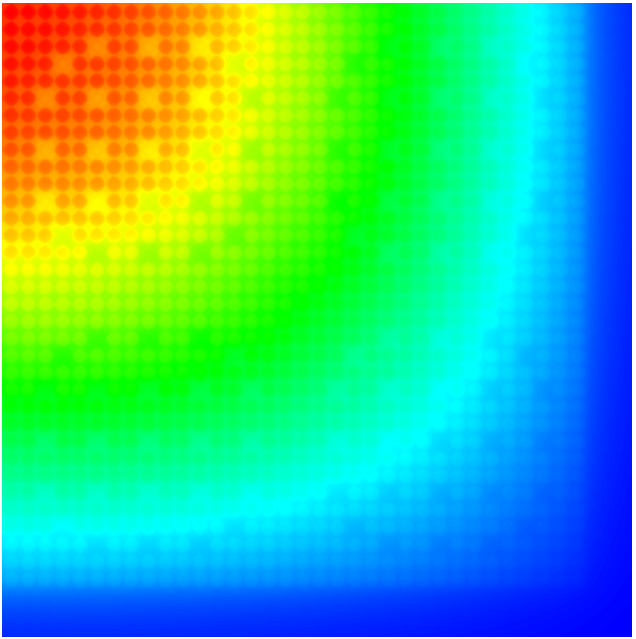
\includegraphics[width=0.350\columnwidth]{images/C5G7_fast.png} \hspace*{3mm}
%{}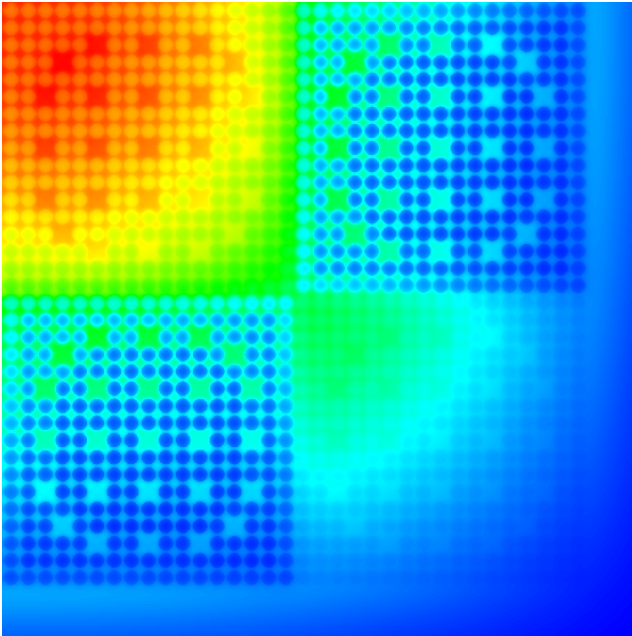
\includegraphics[width=0.350\columnwidth]{images/C5G7_thermal.png}
}
\only<3>
{
\centering
%{}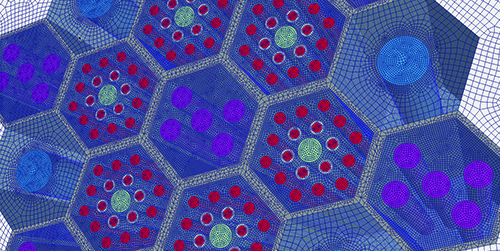
\includegraphics[width=0.70\columnwidth]{images/kitware-cmb-nuke.jpg}
\begin{block}{}{\footnotesize
https://afinemesh.files.wordpress.com/2015/07/kitware-cmb-nuke.jpg
}\end{block}
}
\end{frame}
% --------------------------------------------
\begin{frame}[t]\frametitle{Topics of this Dissertation Work}

\end{frame}
% --------------------------------------------
\begin{frame}[t]\frametitle{The Continuous-Energy Transport Equation} \vspace{-2.5mm}
\begin{block}{Transport Equation}{\footnotesize
\begin{equation*}
\left[ { \bf \Omega} \cdot {\bf \nabla}  + \sigma_t ({\bf r}, E) \right] \psi ({\bf r}, E, {\bf \Omega}) = \int\displaylimits_{4 \pi} \int\displaylimits_{0}^{\infty}  \, \sigma_s ({\bf r}, E' , E, {\bf \Omega}' , {\bf \Omega}) \psi ({\bf r}, E', {\bf \Omega}') d E'  d \Omega'+ Q ({\bf r}, E, {\bf \Omega})
\end{equation*}
}\end{block} \vspace{-1.0mm}
\begin{block}{Boundary Conditions}{\footnotesize
\begin{equation*}
\psi ({\bf r}, E, {\bf \Omega}) = \psi^{inc} ({\bf r}, E, {\bf \Omega}) +  \int\displaylimits_{\vec{\Omega}' \cdot \vec{n} > 0} \int\displaylimits_{0}^{\infty} \beta ({\bf r}, E' , E, {\bf \Omega}' , {\bf \Omega}) \psi ({\bf r}, E', {\bf \Omega}') d E'  d \Omega'
\end{equation*}
}\end{block} \vspace{-1.0mm}
\begin{block}{Term Definitions} {\footnotesize
${\bf r}$ -  neutron position \\
$E$ -  neutron energy \\
${\bf \Omega}$ - neutron solid angle \\
$\psi  ({\bf r}, E, {\bf \Omega})$ - angular flux  \\
$Q  ({\bf r}, E, {\bf \Omega})$ - distributed neutron source \\
$\sigma_t ({\bf r}, E)$ - total macroscopic cross section \\
$\sigma_s ({\bf r}, E' , E, {\bf \Omega}' , {\bf \Omega})$ - total macroscopic scattering cross section\\
$\beta ({\bf r}, E' , E, {\bf \Omega}' , {\bf \Omega})$ - boundary albedo 
}\end{block}
\end{frame}
% --------------------------------------------
\begin{frame}[t]\frametitle{Multigroup DGFEM $S_N$ Transport Equation}

\end{frame}
% --------------------------------------------
\begin{frame}[t]\frametitle{Iterative Procedure}

\begin{block}{Source Iteration} {\small
\begin{equation*}
\begin{aligned}
 \psi^{(\ell+1)} &= {\bf L}^{-1} \left( {\bf M} {\bf \Sigma} \phi^{(\ell)}  +  {\bf Q} \right) \\
\phi^{(\ell+1)} &= {\bf D}  \psi^{(\ell+1)}
\end{aligned}
\end{equation*}
The operation ${\bf L}^{-1}$ is a transport sweep.\\
}
\end{block}

\begin{block}{Operator Terms} {\small
\begin{tabular}{ll}
${\bf L}$ - streaming + collision operator & ${\bf L } = diag(L_1, \ldots, L_{n_\Omega})$ \\
${\bf M}$ - moment-to-discrete operator &
${\bf D}$ - discrete-to-moment operator \\
${\bf \Sigma}$ - scattering operator &
${\bf Q}$ - source operator \\
\end{tabular}
}
\end{block}

\begin{block}{Flux Moment Equivalent Linear System}
\begin{equation*}
{\bf  ( I - DL^{-1} M\Sigma) \Phi = D L^{-1} Q}
\end{equation*}
\end{block}
\end{frame}
% --------------------------------------------
\begin{frame}[t]\frametitle{Polytope Meshes}
         \begin{block}{}{\footnotesize
			\begin{itemize}
				\item <1-> Other physics communities are now employing polytope grids due to decreased cell/face counts (CFD in particular)
				\item <2-> They allow for transition elements between different domain regions
				\item <3-> Hanging nodes from non-conforming meshes are not necessary
				\item <4-> Independently-generated simplicial grids ({\em i.e.} created in parallel) can be stitched together with polytopes without communicating the whole mesh across processors
			\end{itemize}}
         \end{block}
\centering
\only<1>{
\vspace{0.5cm}
{}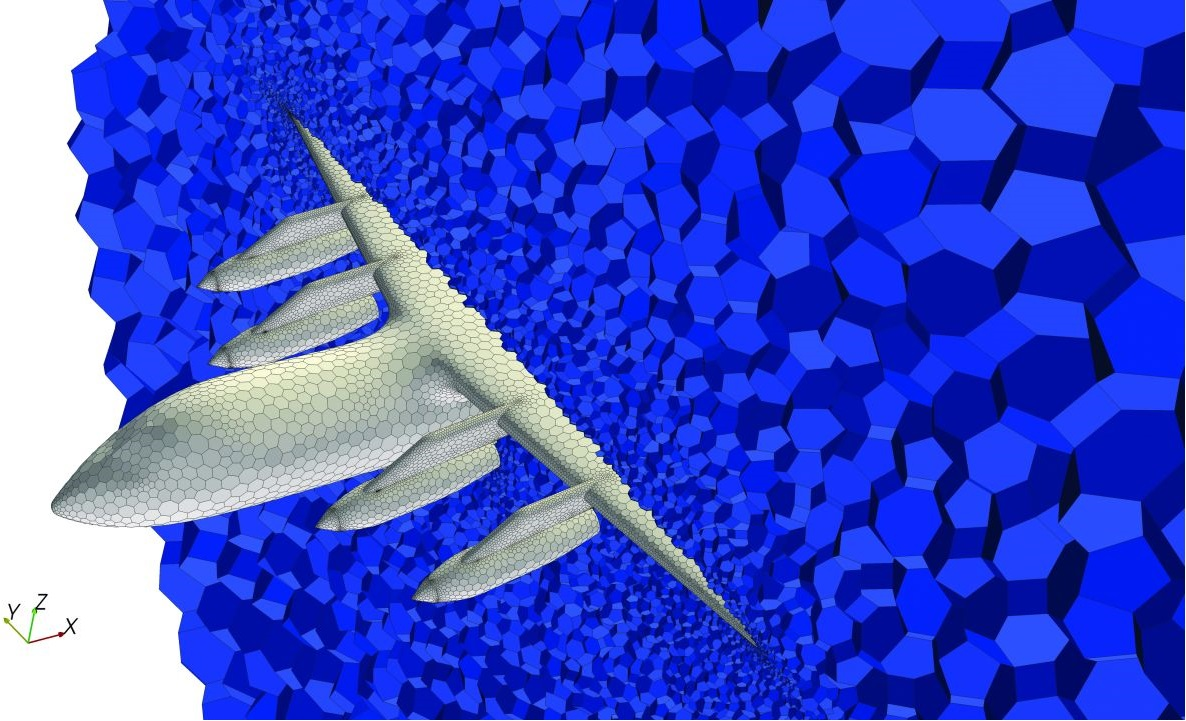
\includegraphics[width=0.45\columnwidth]{images/Polymesh_sized.jpg}
}
\only<2>{
\vspace{0.4cm}
{}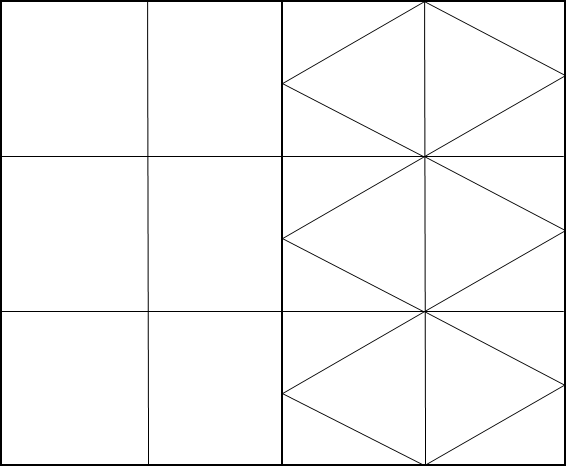
\includegraphics[width=0.4\columnwidth]{images/transition_elements_rev1.png}
}
\only<3>{
\vspace{0.5cm}
{}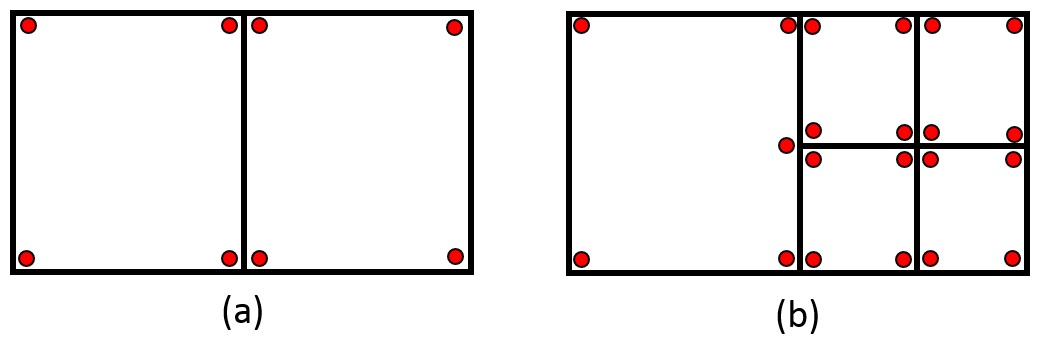
\includegraphics[width=0.65\columnwidth]{images/locally_refined_nodes.png}
}
\only<4>{
\centering
{}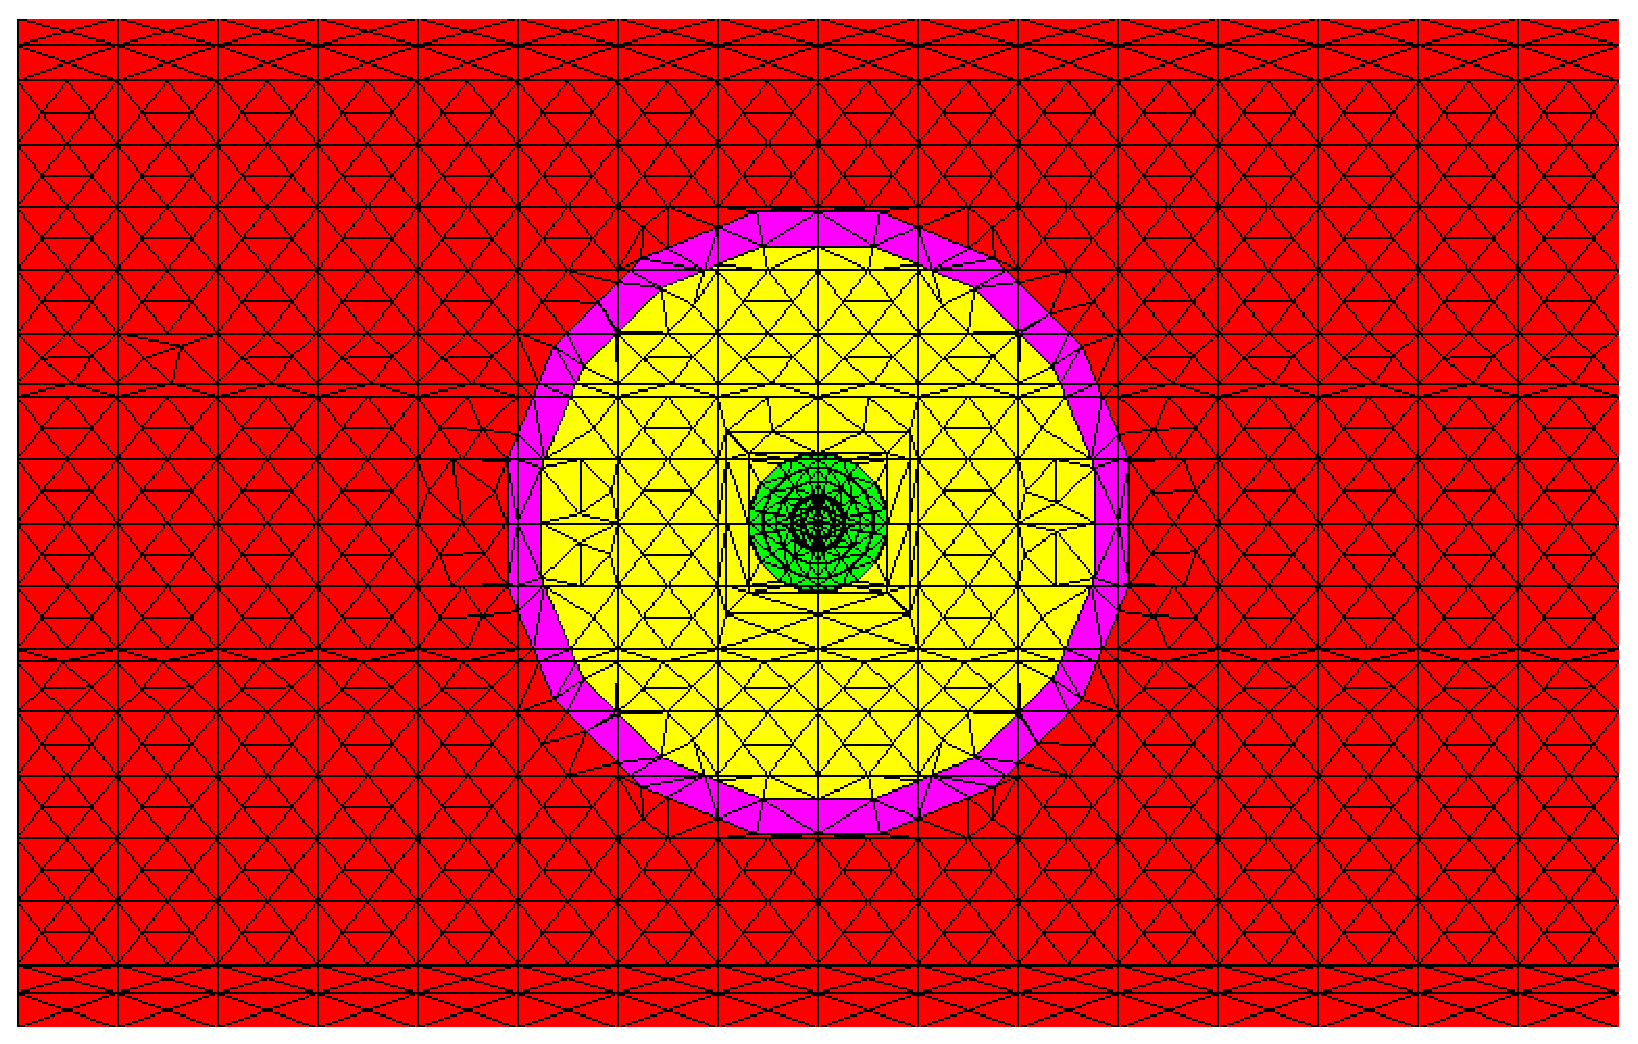
\includegraphics[width=0.52\columnwidth]{images/IM1_30_rot.eps} \hspace{1.0cm}
{}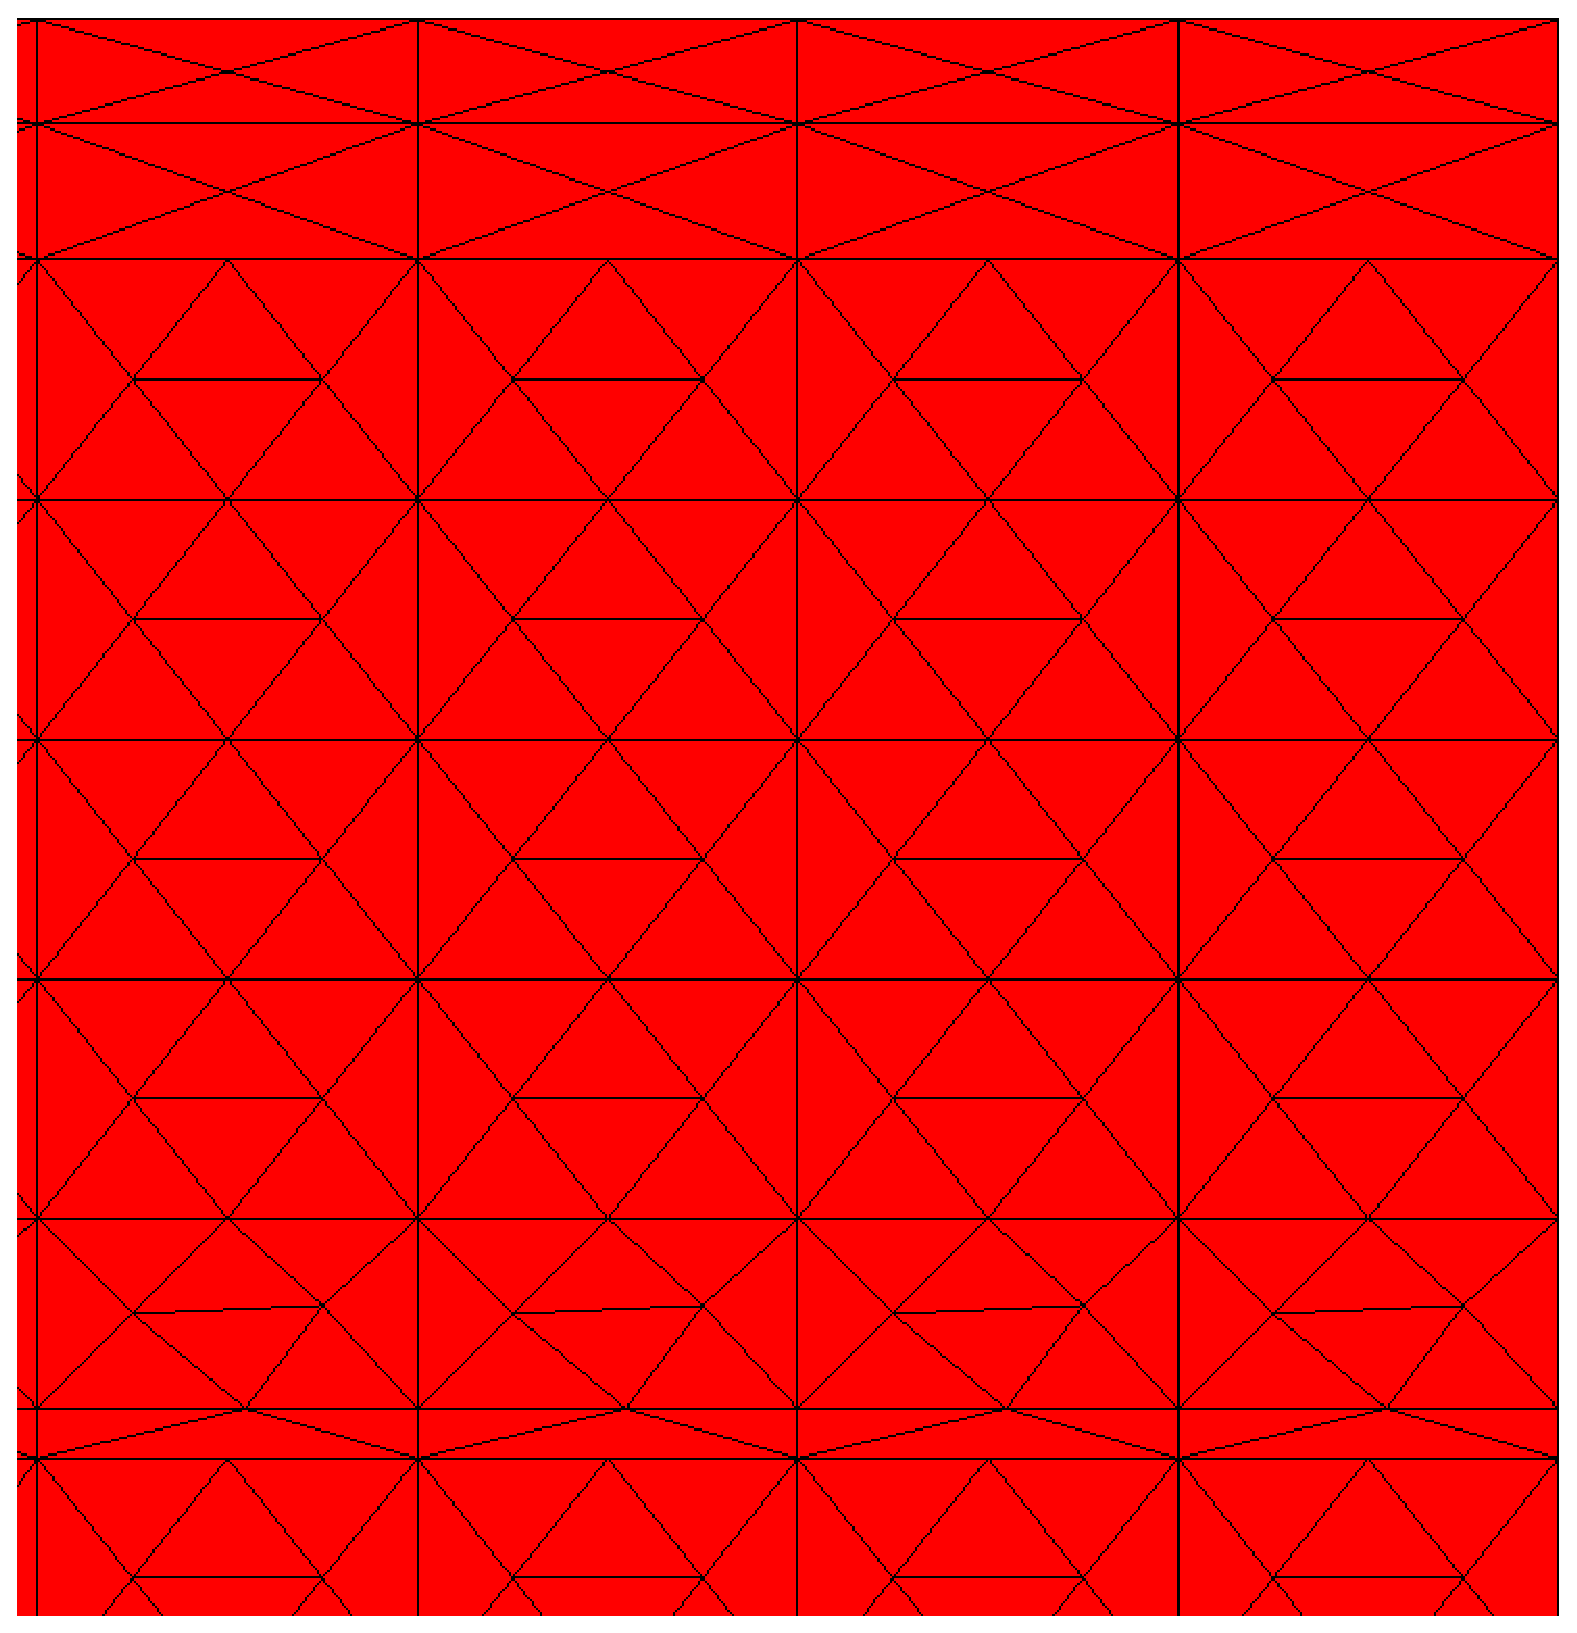
\includegraphics[width=0.345\columnwidth]{images/IM1_zoom.eps}
}
\end{frame}
% --------------------------------------------
\begin{frame}[t]\frametitle{Higher-Order FEM Basis Functions}
\begin{block}{}
\begin{itemize}
\item <1->
\item <2->
\end{itemize}
\end{block}
\centering
\only<1>
{
\centering
\begin{columns}
\column{0.333\textwidth}
\centering
{}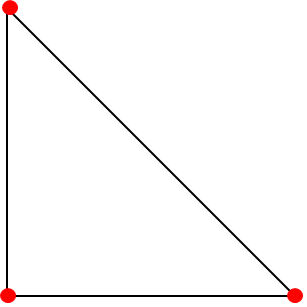
\includegraphics[width=0.75\columnwidth]{images/ref_tri_dofs_k1.png}\\
Linear
\column{0.333\textwidth}
\centering
{}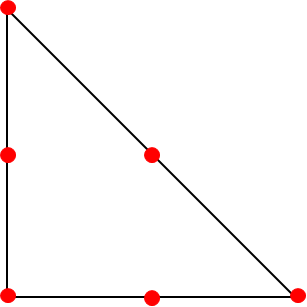
\includegraphics[width=0.75\columnwidth]{images/ref_tri_dofs_k2.png} \\
Quadratic
\column{0.333\textwidth}
\centering
{}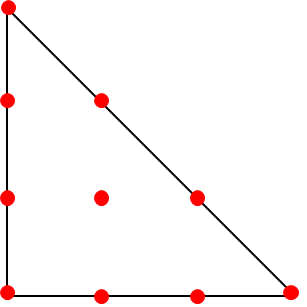
\includegraphics[width=0.75\columnwidth]{images/ref_tri_dofs_k3.png} \\
Cubic
\end{columns}
}
\only<2>
{
{}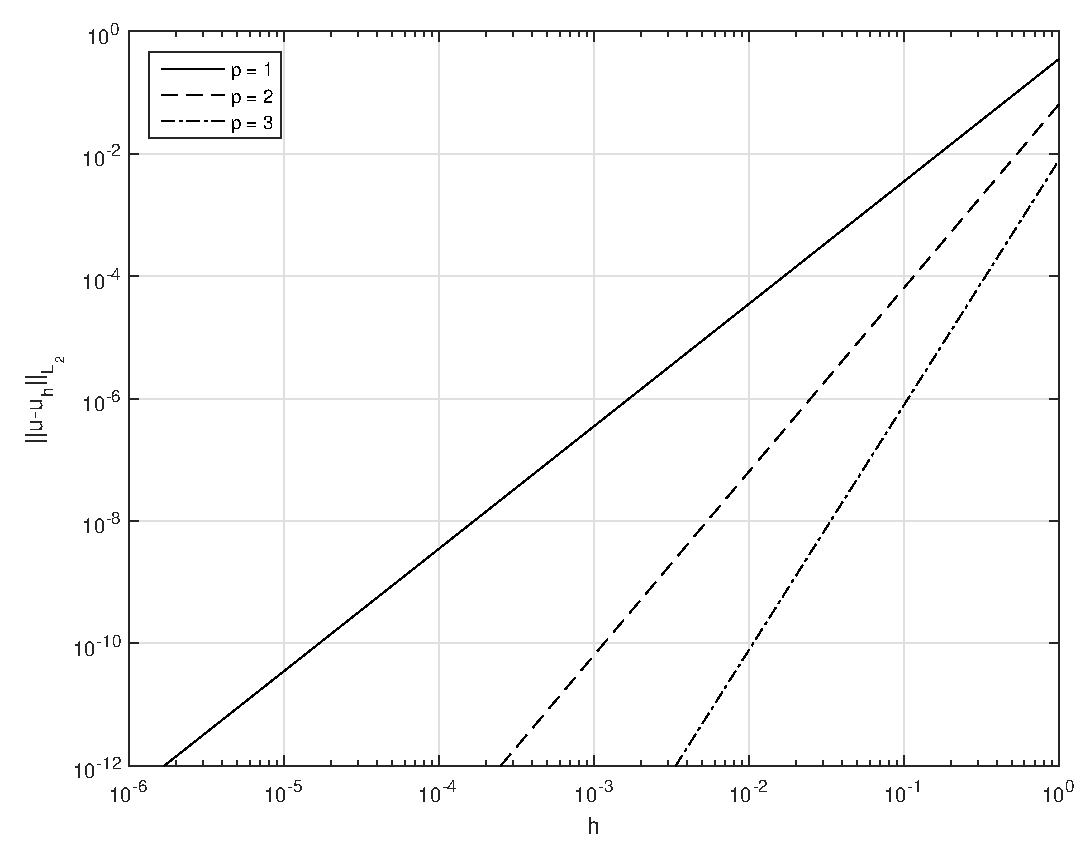
\includegraphics[width=0.475\columnwidth]{images/hConverge.eps} \hspace*{1mm}
{}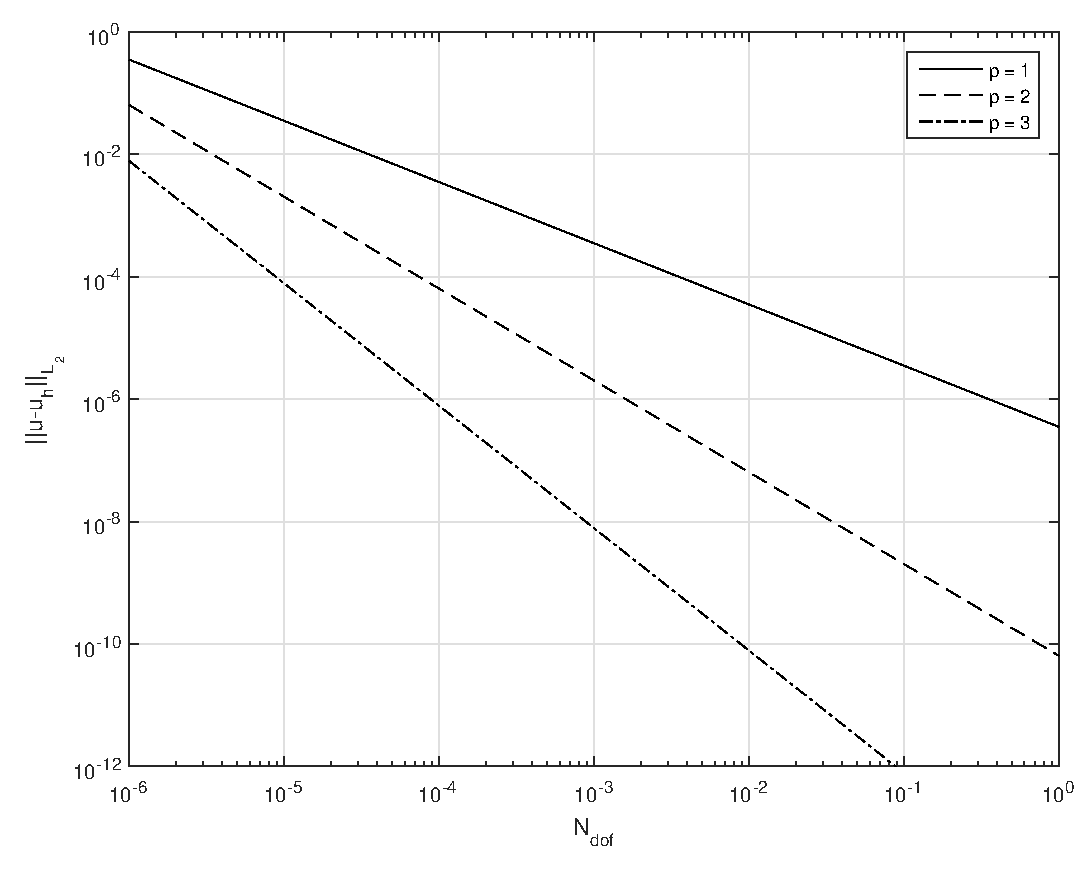
\includegraphics[width=0.475\columnwidth]{images/NConverge.eps}
}
\end{frame}
% --------------------------------------------
\begin{frame}[t]\frametitle{Diffusion Synthetic Acceleration}
\only<1-2>{
\begin{block}{Source Iteration Approximate Spectral Radius}
\begin{equation*}
\rho^{(k+1)} \approx \frac{||  \phi^{(k+1)} -  \phi^{(k)} ||}{||  \phi^{(k)} -  \phi^{(k-1)}  ||} 
\end{equation*}
\end{block}
\begin{block}{Optically Thick Cases - leakage/absorption does not dominate}{\small
\begin{itemize}
	\item $\sigma_s^{g \rightarrow g} / {\sigma_{t,g}} \approx  1$ and $\left( \sigma_{t,g} \cdot \text{diam} (\mathcal{D}) \right) \gg 1$
	\item Thermal upscattering into higher energy groups is significant
\end{itemize}}
\end{block}
}
\onslide<2->{
\begin{block}{Answer - Precondition the transport sweep}{\small
\begin{itemize}
	\item Diffusion Synthetic Acceleration (DSA)
	\item Transport Synthetic Acceleration (TSA)
	\item Boundary Projection Acceleration (BPA)
	\item etc.
\end{itemize}
}\end{block}
}
\end{frame}
% --------------------------------------------
%%%%%%%%%%%%%%%%%%%%%%%%%%%%%%%%%%%%%%%%%%%%%%%%%%%%%%%%%%%%%%%%%%%%%%%%%%%%%%%%%%%%%%%%%%%%%%
%%%%%%%%%%%%%%%%%%%%%%%%%%%%%%%%%%%%%%%%%%%%%%%%%%%%%%%%%%%%%%%%%%%%%%%%%%%%%%%%%%%%%%%%%%%%%%
\typeout{***********************************************************************************}
\typeout{POLYFEM}
%%%%%%%%%%%%%%%%%%%%%%%%%%%%%%%%%%%%%%%%%%%%%%%%%%%%%%%%%%%%%%%%%%%%%%%%%%%%%%%%%%%%%%%%%%%%%%
% POLYFEM SECTION
\section{POLYFEM}
%%%%%%%%%%%%%%%%%%%
\subsection{}
%%%%%%%%%%%%%%%%%%%
%---------------------------
\setbeamerfont{frametitle}{size=\normalsize}
\begin{frame}[t]\frametitle{Polytope Finite Elements}
\centering
\begin{block}{2D arbitrary convex/concave polygons}
\centering
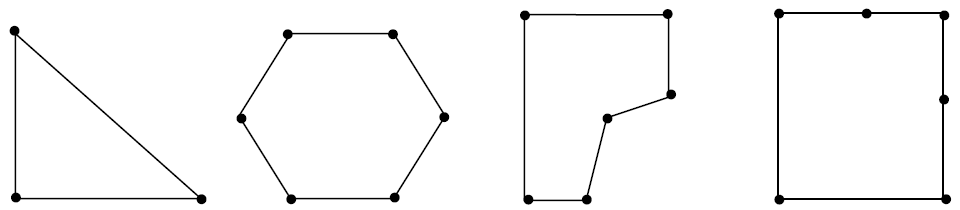
\includegraphics[width=0.70\textwidth]{images/arbitrary_polygons.png}
\end{block}
\vspace{0.5cm}
\begin{block}{3D convex polyhedra}
\centering
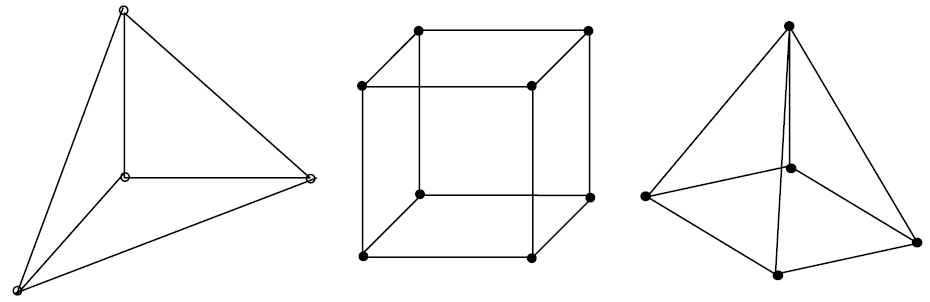
\includegraphics[width=0.70\textwidth]{images/arbitrary_polyhedra.png}
\end{block}
\end{frame}
% --------------------------------------------
\begin{frame}[t]\frametitle{Finite element architecture}
\begin{block}{Mass Matrix - element $K$}
\begin{equation*}
{\bf M}^K = \int_{K} d\vec{r} \, \lambda (\vec{x}) \, \lambda^T (\vec{x})  =  \sum\displaylimits_{q=1}^{N_q^K} w_q^K \, \lambda (\vec{x}_q^K) \, \lambda^T (\vec{x}_q^K) 
\end{equation*}
\end{block}
\begin{block}{Advection Matrix - element $K$}
\begin{equation*}
{\bf G}^K = \int_{K} d\vec{r} \, \vec{\nabla} \lambda (\vec{x}) \, \lambda^T (\vec{x}) = \sum\displaylimits_{q=1}^{N_q^K}  w_q^K \, \vec{\nabla} \lambda (\vec{x}_q^K) \, \lambda^T (\vec{x}_q^K) 
\end{equation*}
\end{block}
\begin{block}{Surface Matrix - face $f$ for element $K$}
\begin{equation*}
{\bf N}_f^K = \int_{f} ds \, \lambda (\vec{x}) \, \lambda^T (\vec{x})  = \sum\displaylimits_{q=1}^{N_f}  w_q^f \, \lambda (\vec{x}_q^f) \, \lambda^T (\vec{x}_q^f) 
\end{equation*}
\end{block}
\end{frame}
% --------------------------------------------
%%%%%%%%%%%%%%%%%%%
\subsection{Linear Basis Functions on Polygons}
%%%%%%%%%%%%%%%%%%%
% --------------------------------------------
\begin{frame}[t]\frametitle{Linear Basis Functions - Generalized Barycentric Coordinates}
\centering
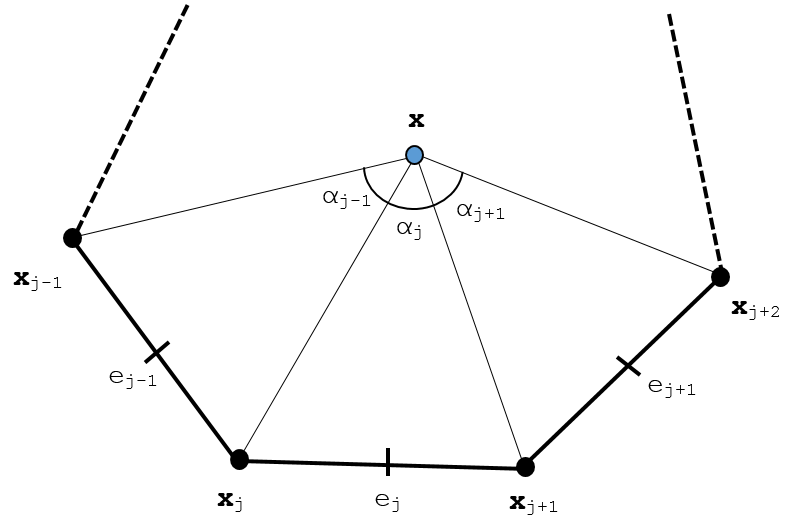
\includegraphics[width=0.35\textwidth]{images/ref_polygon.png}
\only<1>{
\begin{block}{Basis Function Properties - Barycentric Coordinates}{\small
$\lambda_i$ - linear basis function located at vertex $i$ \vspace{0.25cm}
\vspace{-1mm}
	\begin{enumerate}
	\item Positivity*: $\lambda_i \geq 0$ \vspace{1mm}
	\item Partition of Unity: $\sum_i \lambda_i = 1$ \vspace{1mm}
	\item Affine combination: $\sum_i \vec{x}_i \lambda_i (\vec{x}) = \vec{x}$ \vspace{1mm}
	\item Lagrange property: $\lambda_i (\vec{x}_j) = \delta_{ij}$ 
	\item Piecewise boundary linearity: $\lambda_j ((1-\mu ) \vec{x}_j  + \mu \vec{x}_{j+1})  = (1-\mu ) \lambda_j (\vec{x}_j ) + \mu \lambda_j (\vec{x}_{j+1} )$
	\end{enumerate}
\vspace{1mm}
*convex polygons
}\end{block}
}
\only<2>{
\begin{block}{Linear basis functions that we consider}
	\begin{enumerate}
	\item Wachspress rational coordinates*
	\item Piecewise linear (PWL) coordinates*
	\item Mean value coordinates
	\item Maximum entropy coordinates
	\end{enumerate}
\vspace{2mm}
*have been previously analyzed for transport problems
\end{block}
}
\end{frame}
% --------------------------------------------
\begin{frame}[t]\frametitle{Wachspress Rational Functions}
\centering
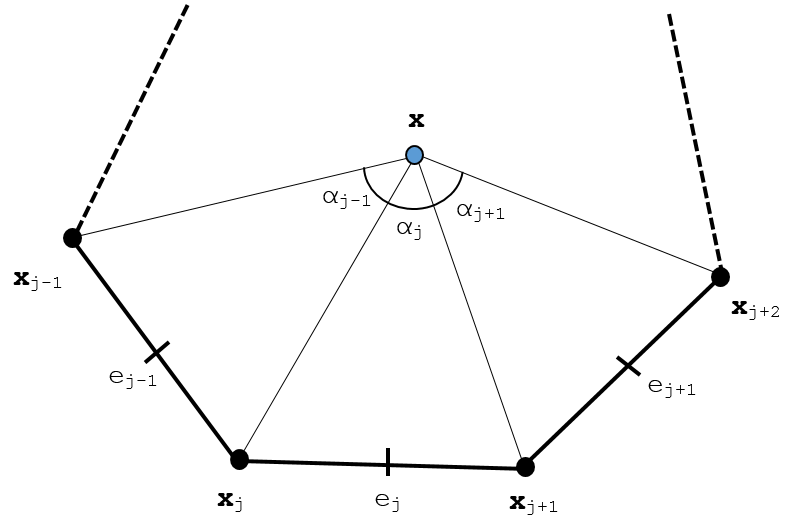
\includegraphics[width=0.40\textwidth]{images/ref_polygon.png}
\vspace{0.3cm}
\begin{block}{}
\begin{equation*}
\lambda_i^W (\vec{x}) = \frac{w_i (\vec{x}) }{ \sum_{j} w_j (\vec{x})}, \qquad w_j (\vec{x}) = \frac{A(\vec{x}_{j-1}, \vec{x}_{j}, \vec{x}_{j+1})}{A(\vec{x}, \vec{x}_{j-1}, \vec{x}_{j}) \, A(\vec{x}, \vec{x}_{j}, \vec{x}_{j+1})}
\end{equation*}
\end{block}
\begin{block}{}
\begin{equation*}
A(\vec{x}_1, \vec{x}_{2}, \vec{x}_{3}) = \frac{1}{2} \left|
\begin{array}{ccc}
1 & 1 & 1 \\
x_1 & x_2 & x_3 \\
y_1 & y_2 & y_3
\end{array} \right|
\end{equation*}
\end{block}
\end{frame}
% --------------------------------------------
\begin{frame}[t]\frametitle{Piecewise Linear (PWL) Functions}
\centering
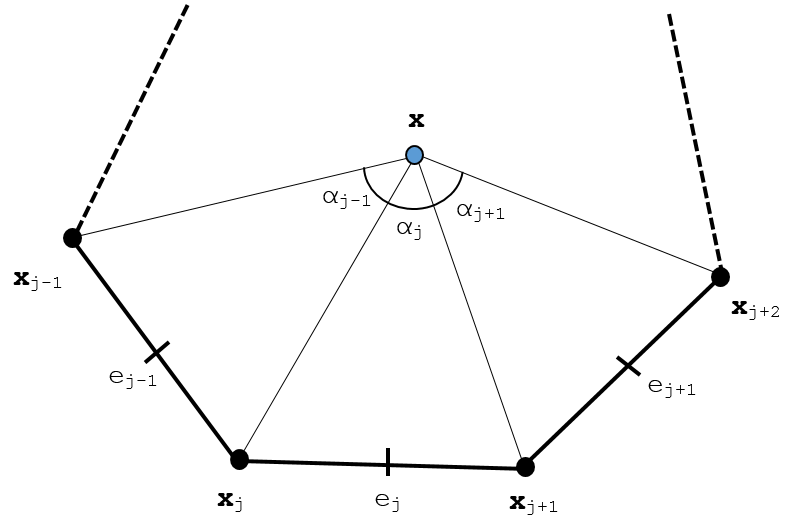
\includegraphics[width=0.40\textwidth]{images/ref_polygon.png}
\vspace{0.3cm}
\begin{block}{}
\begin{equation*}
\lambda_i^{PWL} (\vec{x}) =  t_i (\vec{x}) + \alpha_i t_c (\vec{x})
\end{equation*}
\end{block}
\begin{block}{}
$t_i $ - standard 2D linear function for a triangle $(i,i+1,C)$; 1 at vertex $i$ that linearly decreases to 0 to the cell center and the adjoining vertices \\ \vspace{1mm}
$t_c$ - 2D tent function; 1 at cell center and linearly decreases to 0 to each cell vertex \\ \vspace{1mm}
$\alpha_i = \frac{1}{N_V}$ - weight parameter for vertex $i$ \\ \vspace{1mm}
$N_V$ - number of cell vertices
\end{block}
\end{frame}
% --------------------------------------------
\begin{frame}[t]\frametitle{Mean Value (MV) Coordinates}
\centering
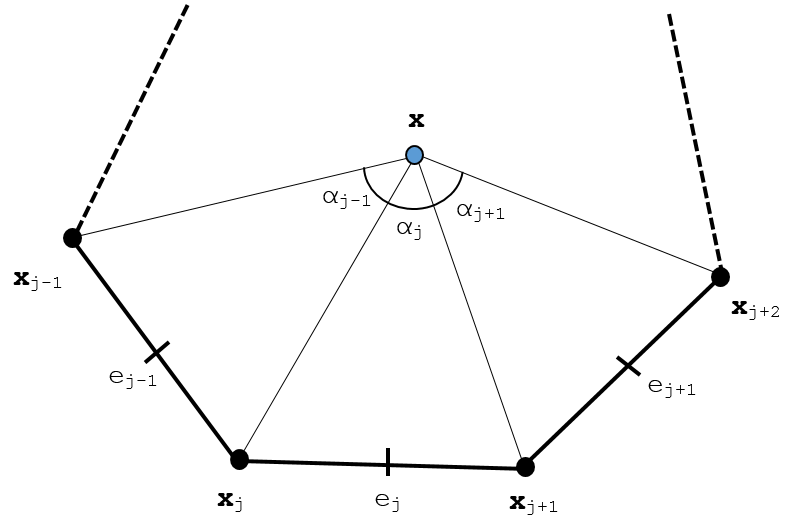
\includegraphics[width=0.40\textwidth]{images/ref_polygon.png}
\vspace{0.3cm}
\only<1>{
\begin{block}{Preserve piecewise linear harmonic maps over triangulations}
\begin{equation*}
\frac{\partial^2 u}{\partial x^2} + \frac{\partial^2 u}{\partial y^2} = 0, \qquad u(\vec{r}) = u_0 , \, \vec{r} \in \partial \mathcal{D} 
\end{equation*} \\
\vspace{1.0cm}
$u(\vec{r})$ - piecewise linear function on the cell boundary
\end{block}
}
\only<2>{
\begin{block}{}
\begin{equation*}
\lambda_i^{MV} (\vec{x}) = \frac{w_i (\vec{x}) }{ \sum_{j} w_j (\vec{x})}, \qquad w_j (\vec{x}) = \frac{\tan(\alpha_{j-1} / 2) + \tan(\alpha_j / 2)}{|\vec{x}_j - \vec{x}|}
\end{equation*}
\end{block}
\begin{block}{Limit as $\vec{x} \rightarrow \vec{x}_j$}
\vspace{-0.25cm}
\begin{columns}
\column{0.5\textwidth}
\centering
\begin{equation*}
\lim_{\vec{x} \rightarrow \vec{x}_j} \tan(\alpha_{j-1} / 2) + \tan(\alpha_j / 2) = 0
\end{equation*}
\column{0.1\textwidth}
\centering
$\longrightarrow$
\column{0.4\textwidth}
\centering
\begin{equation*}
\lim_{\vec{x} \rightarrow \vec{x}_j}  w_j (\vec{x}) = 1
\end{equation*}
\end{columns}
\end{block}
}
\end{frame}
% --------------------------------------------
\begin{frame}[t]\frametitle{Maximum Entropy (ME) Coordinates}
\centering
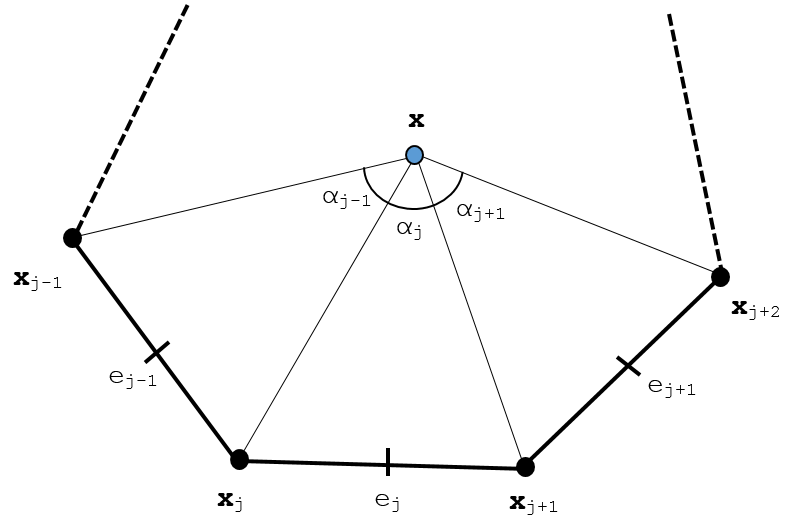
\includegraphics[width=0.40\textwidth]{images/ref_polygon.png}
\vspace{0.3cm}
\only<1>{
\begin{block}{Constrained optimization problem - Shannon Entropy}
\begin{equation*}
\max\displaylimits_{\lambda(\vec{x})}  H(\lambda, m), \qquad  H(\lambda, m) = - \sum\displaylimits_{i} \lambda_i (\vec{x}) \ln \left(   \frac{\lambda_i(\vec{x})}{m_i(\vec{x})} \right)
\end{equation*} \\ \vspace{3mm}
\begin{equation*}
\sum\displaylimits_{i} \lambda_i (\vec{x}) = 1, \qquad \sum\displaylimits_{i} \lambda_i (\vec{x}) ( \vec{x}_i - \vec{x} ) = \vec{0}
\end{equation*}
\end{block}
}
\only<2>{
\begin{block}{}
\begin{equation*}
\lambda_i^{ME} (\vec{x}) = \frac{w_i (\vec{x}) }{ \sum_{j} w_j (\vec{x})}, \qquad w_j (\vec{x}) = m_j(\vec{x}) \exp(- \omega^* \cdot (\vec{x}_j - \vec{x}))
\end{equation*}
\end{block}
\begin{block}{}{\small
\begin{equation*}
\mathcal{L} (\lambda, \omega_0, \omega) = - \sum\displaylimits_{i} \lambda_i (\vec{x}) \ln \left(   \frac{\lambda_i(\vec{x})}{m_i(\vec{x})} \right) - \omega_0 \left(  \sum\displaylimits_{i}  \lambda_i (\vec{x}) -1  \right) - \omega \cdot  \left(  \sum\displaylimits_{i}  \lambda_i (\vec{x}) (\vec{x}_i - \vec{x})  \right)
\end{equation*}}
\end{block}
}
\only<3>{
\begin{block}{}
\begin{equation*}
\lambda_i^{ME} (\vec{x}) = \frac{w_i (\vec{x}) }{ \sum_{j} w_j (\vec{x})}, \qquad w_j (\vec{x}) = m_j(\vec{x}) \exp(- \omega^* \cdot (\vec{x}_j - \vec{x}))
\end{equation*}
\end{block}
\begin{block}{}
\begin{equation*}
\omega^* = \text{argmin} \, F(\omega, \vec{x})  \qquad F(\omega, \vec{x}) = \ln \left(  \sum_j w_j (\vec{x})  \right)
\end{equation*}
\end{block}
}
\end{frame}
% --------------------------------------------
\begin{frame}[t]
\only<1>
{
\frametitle{Summary of the Linear Basis Functions}
\centering
\vspace{1cm}
\begin{table}
\footnotesize
\begin{tabular}{|c|c|c|c|c|}
\hline
Basis Function & Dimension & Polytope Types & Integration & Direct/Iterative \\
\hline \hline
Wachspress	&2D/3D&	Convex*&	Numerical	&Direct\\ \hline
PWL&	1D/2D/3D&	Convex/Concave&	Analytical	&Direct\\ \hline
Mean Value&	2D**&	Convex/Concave&	Numerical	&Direct\\ \hline
Max Entropy&	1D/2D/3D	&Convex/Concave&	Numerical&	Iterative***\\ \hline
\end{tabular}
\end{table}
\vspace{0.5cm}
\begin{block}{}
* - weak convexity for Wachspress coordinates does not cause blow up\\
** - mean value 3D analogue only applicable triangular-faceted polyhedra \\
*** - maximum entropy minimization solved via Newton's Method 
\end{block}
}
\only<2>
{
\frametitle{Basis Functions on the Unit Square}
\begin{columns}
\column{0.50\textwidth}
\centering
{}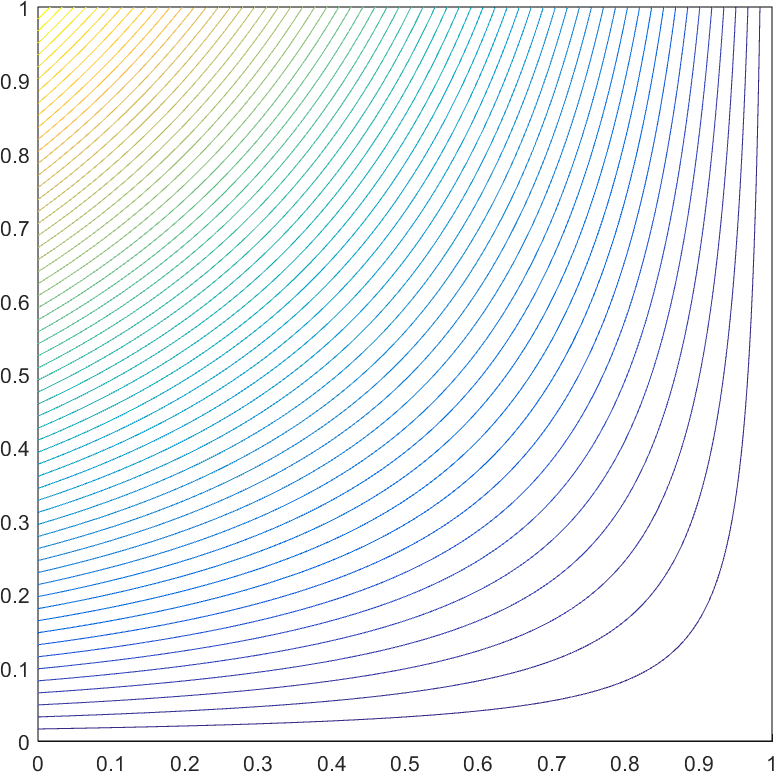
\includegraphics[width=0.55\columnwidth]{images/square_WACHSPRESS1_contour_b4.png} \\
Wachspress\\ \vspace{3mm}
{}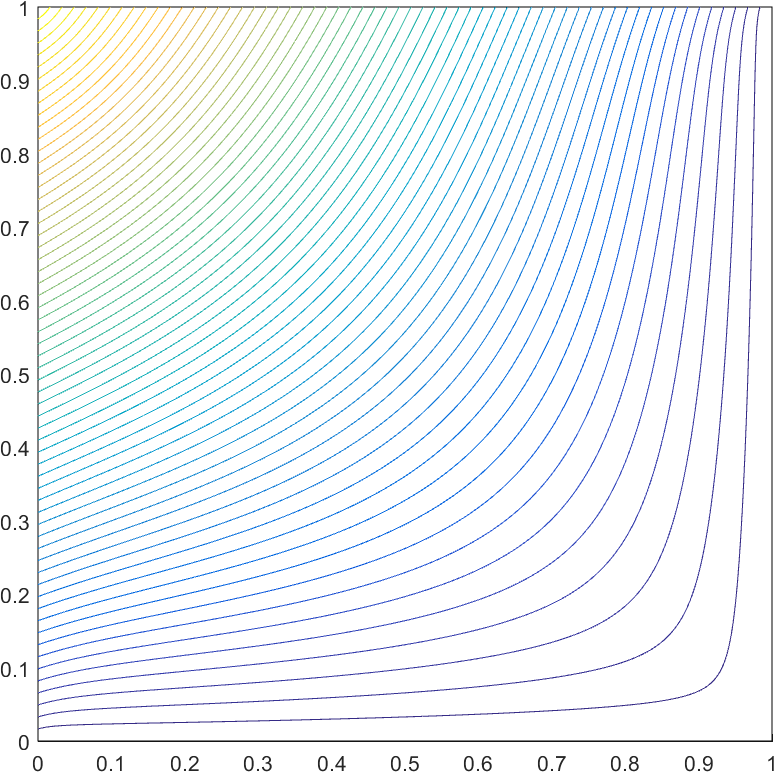
\includegraphics[width=0.55\columnwidth]{images/square_MV1_contour_b4.png} \\
Mean Value
\column{0.50\textwidth}
\centering
{}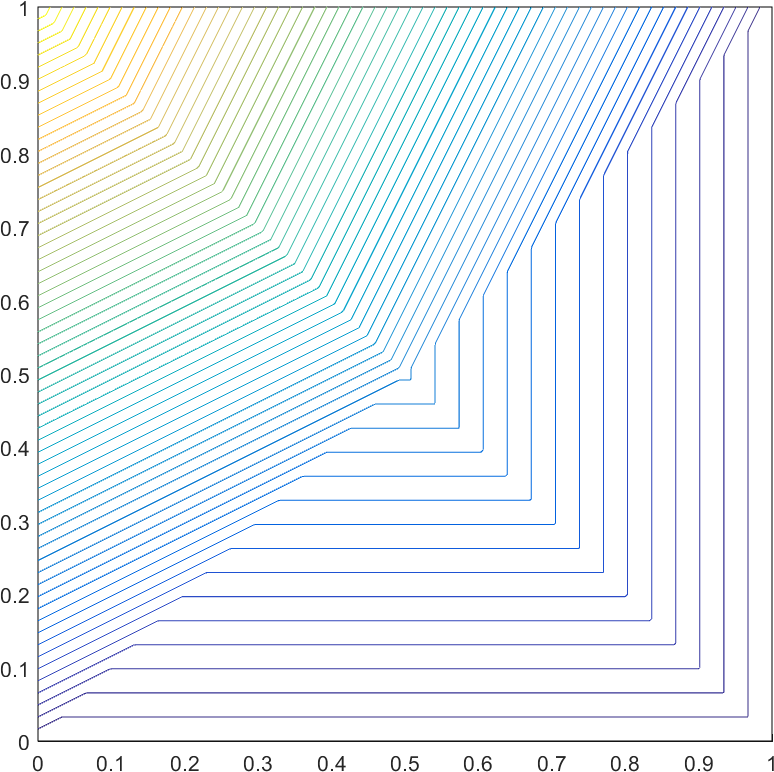
\includegraphics[width=0.55\columnwidth]{images/square_PWLD1_contour_b4.png} \\
PWL\\ \vspace{3mm}
{}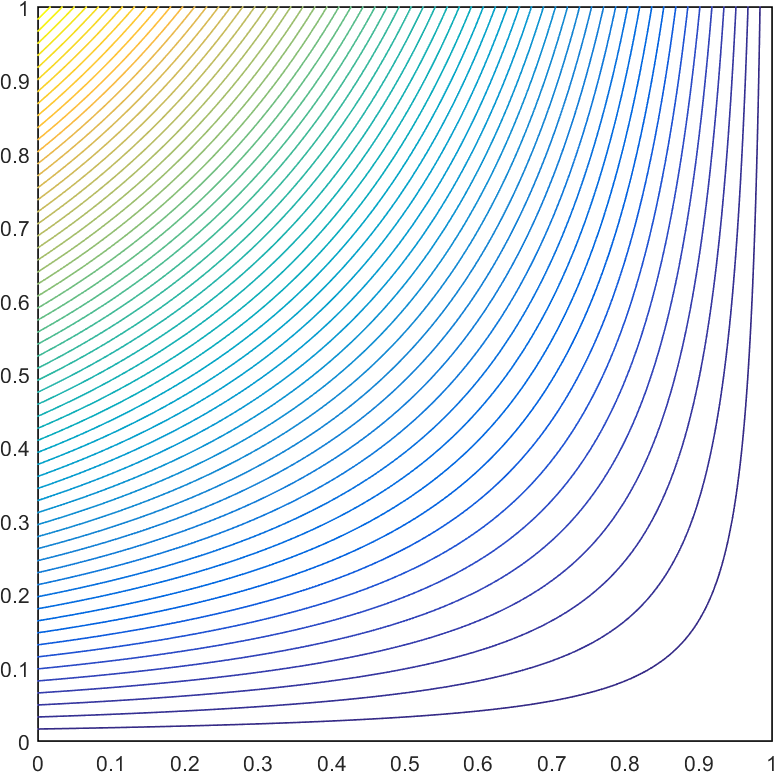
\includegraphics[width=0.55\columnwidth]{images/square_MAXENT1_contour_b4.png} \\
Maximum Entropy
\end{columns}
}
\only<3>
{
\frametitle{Basis Functions on the Degenerate Pentagon}
\begin{columns}
\column{0.50\textwidth}
\centering
{}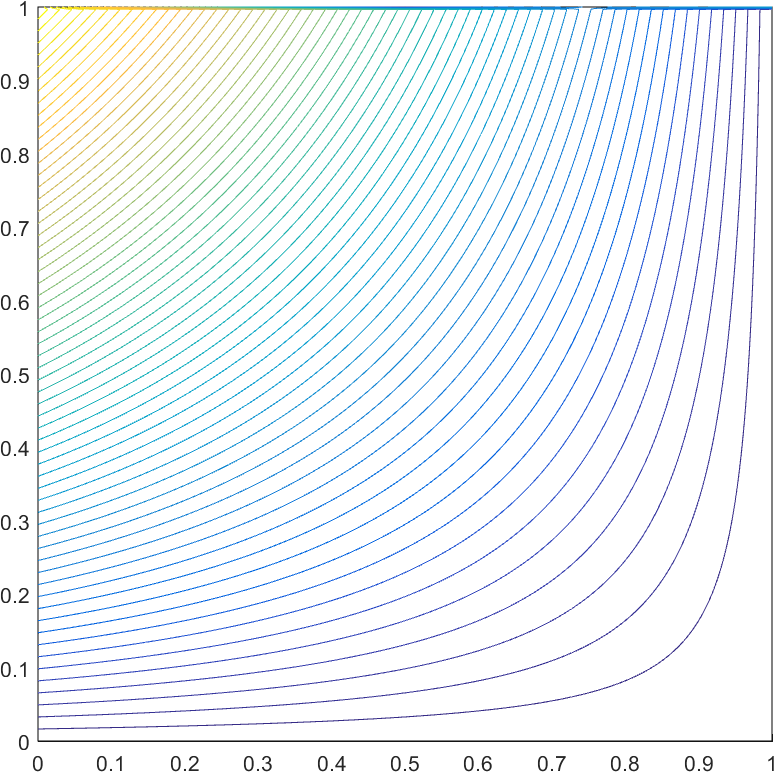
\includegraphics[width=0.55\columnwidth]{images/deg_square_WACHSPRESS1_contour_b5.png} \\
Wachspress\\ \vspace{3mm}
{}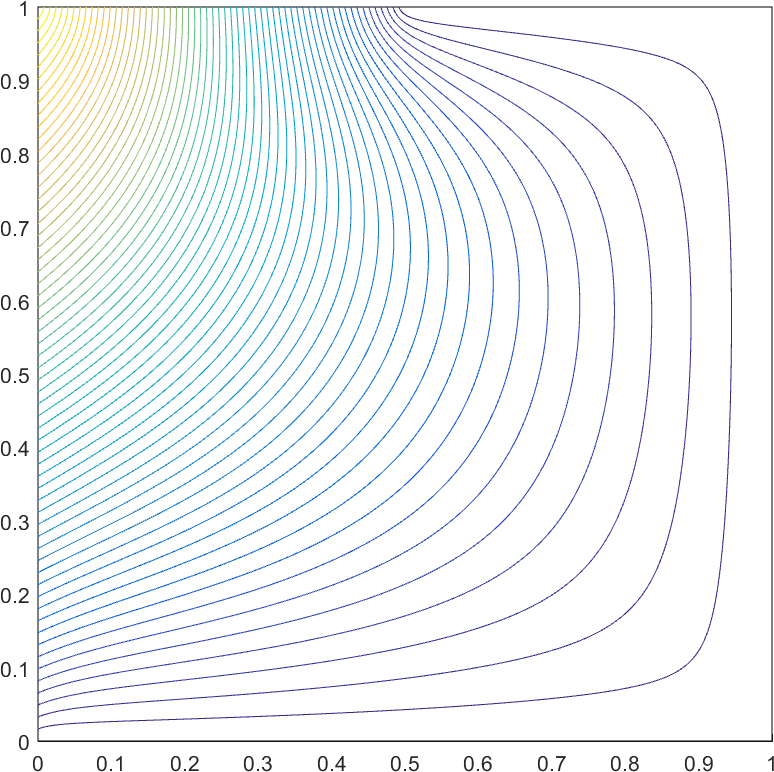
\includegraphics[width=0.55\columnwidth]{images/deg_square_MV1_contour_b5.png} \\
Mean Value
\column{0.50\textwidth}
\centering
{}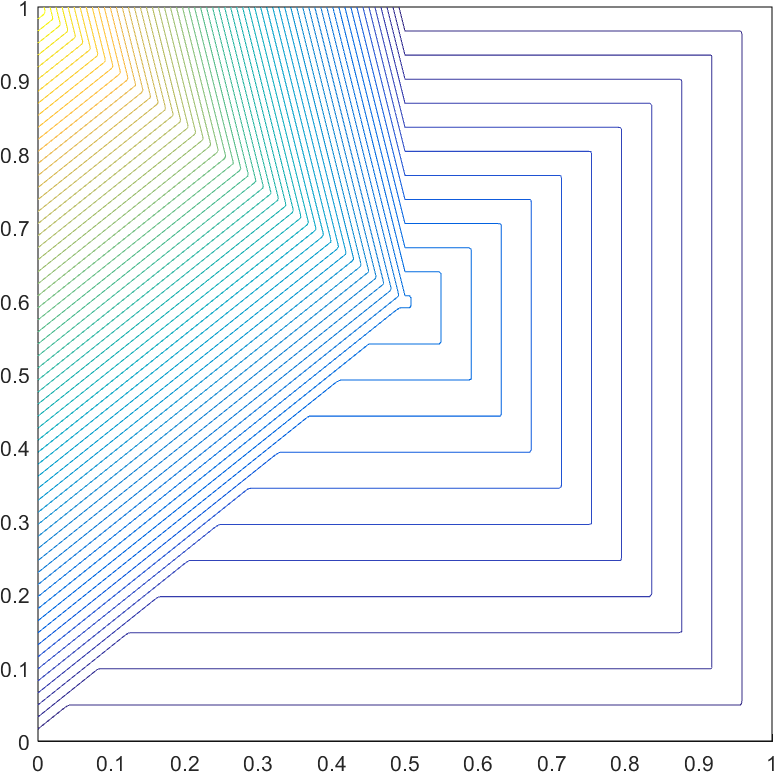
\includegraphics[width=0.55\columnwidth]{images/deg_square_PWLD1_contour_b5.png} \\
PWL\\ \vspace{3mm}
{}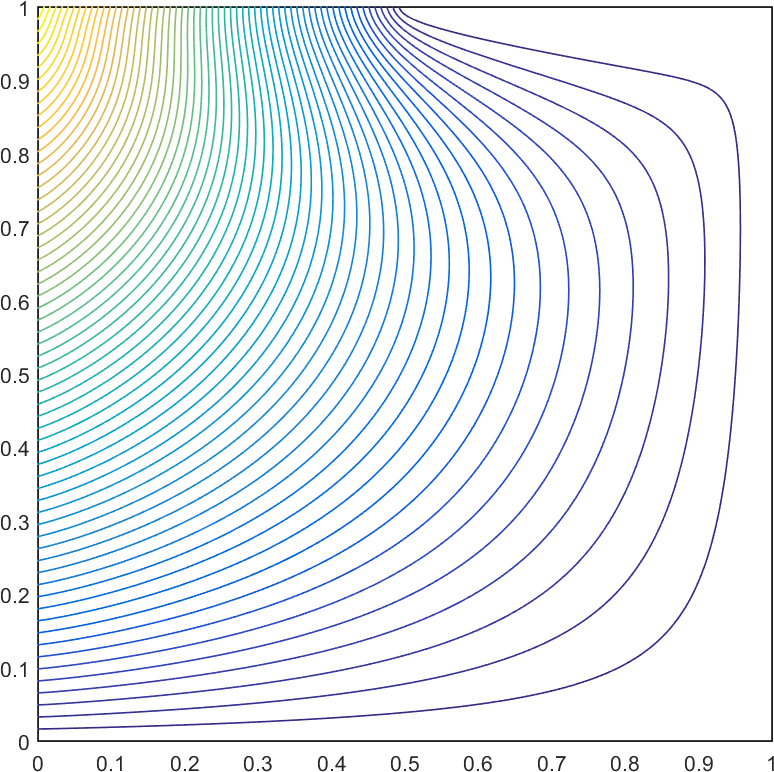
\includegraphics[width=0.55\columnwidth]{images/deg_square_MAXENT1_contour_b5.png} \\
Maximum Entropy
\end{columns}
}
\only<4>
{
\frametitle{Basis Functions on the Degenerate Pentagon}
\begin{columns}
\column{0.50\textwidth}
\centering
{}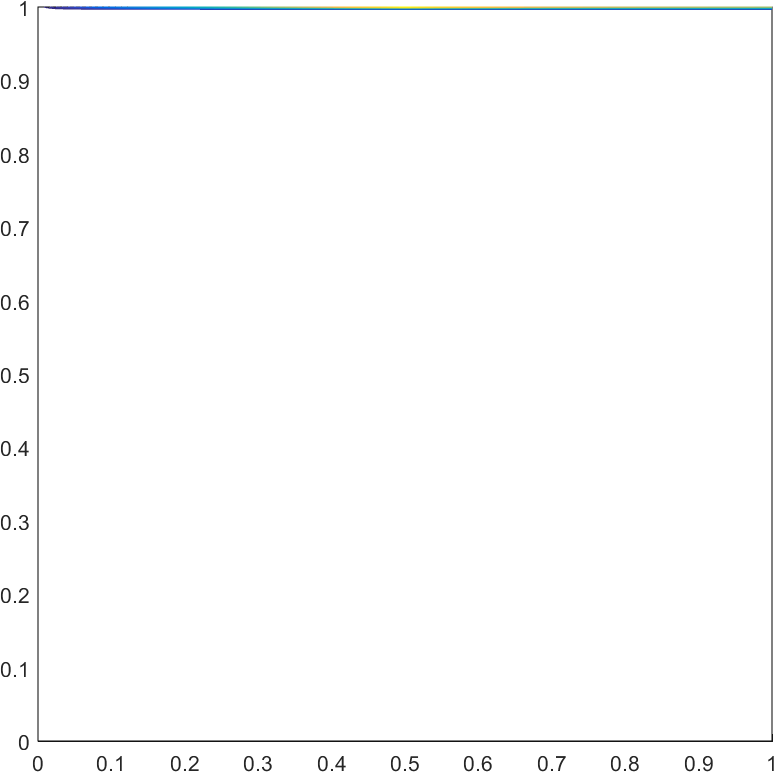
\includegraphics[width=0.55\columnwidth]{images/deg_square_WACHSPRESS1_contour_b4.png} \\
Wachspress\\ \vspace{3mm}
{}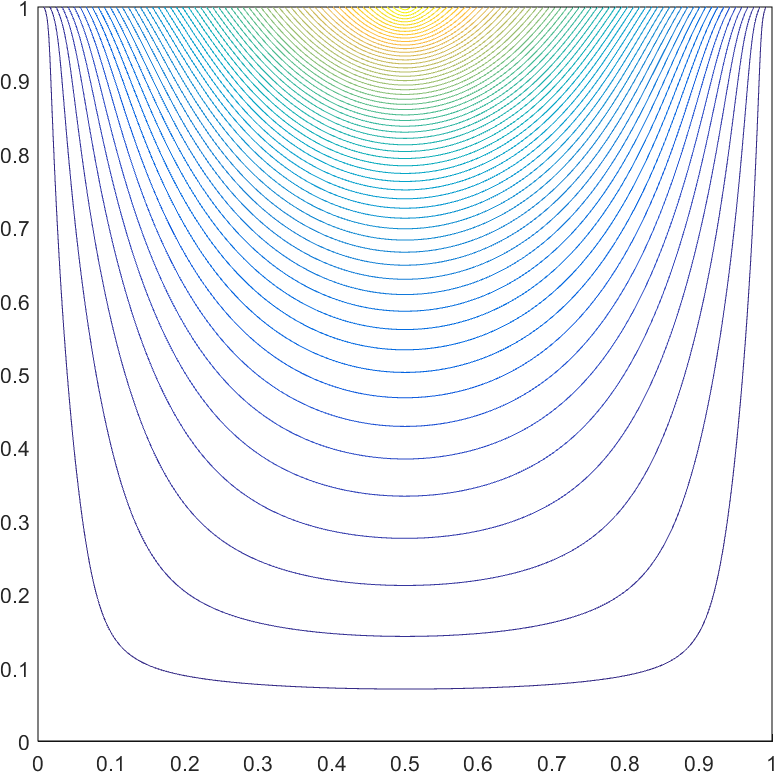
\includegraphics[width=0.55\columnwidth]{images/deg_square_MV1_contour_b4.png} \\
Mean Value
\column{0.50\textwidth}
\centering
{}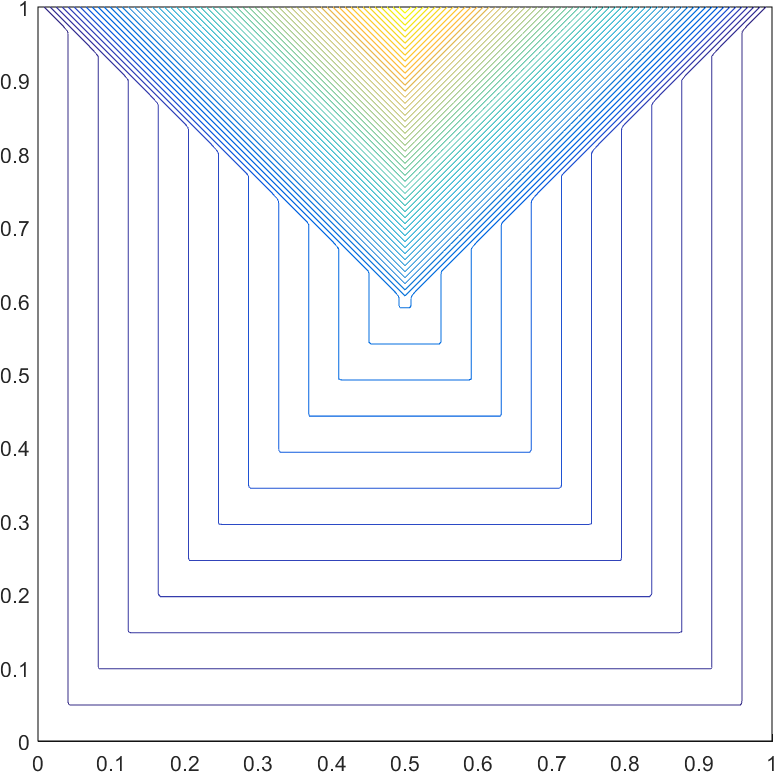
\includegraphics[width=0.55\columnwidth]{images/deg_square_PWLD1_contour_b4.png} \\
PWL\\ \vspace{3mm}
{}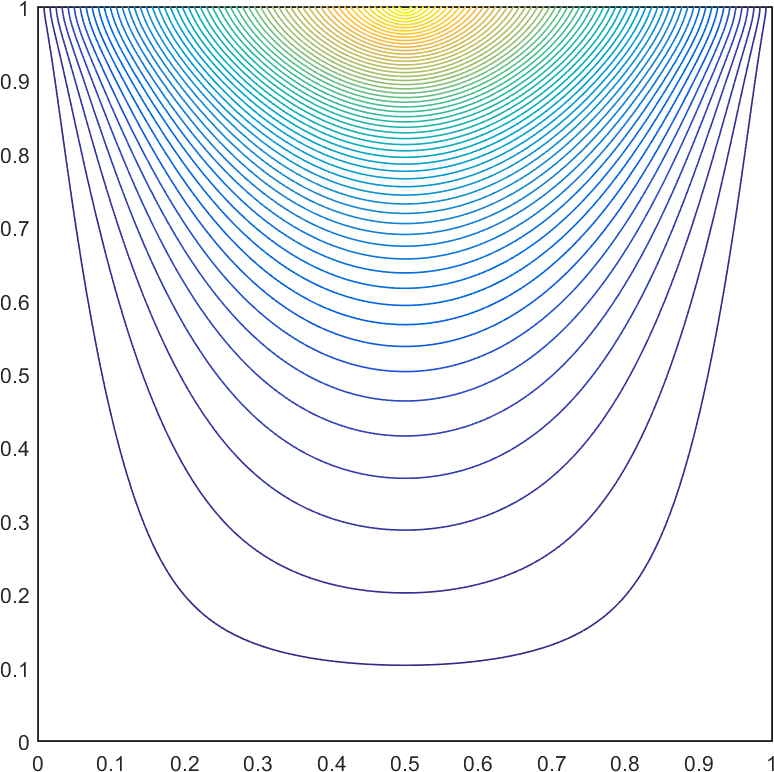
\includegraphics[width=0.55\columnwidth]{images/deg_square_MAXENT1_contour_b4.png} \\
Maximum Entropy
\end{columns}
}
\only<5>
{
\frametitle{Basis Functions on the L-Shaped Domain}
%\vspace{1cm}
\begin{columns}
\column{0.333\textwidth}
\centering
{}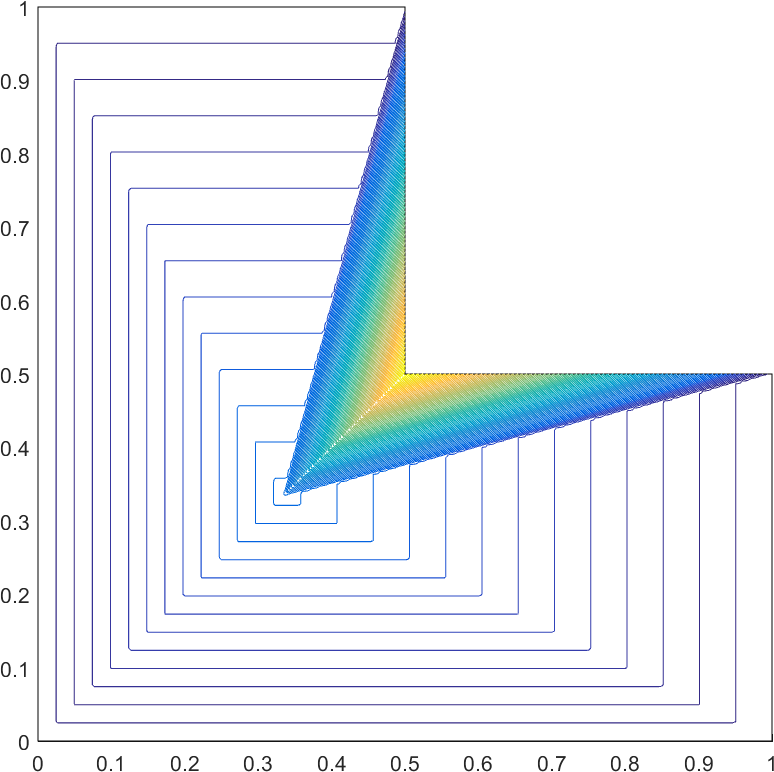
\includegraphics[width=0.85\columnwidth]{images/L-domain_PWLD1_contour_b4.png} \\
\vspace{3mm}
{}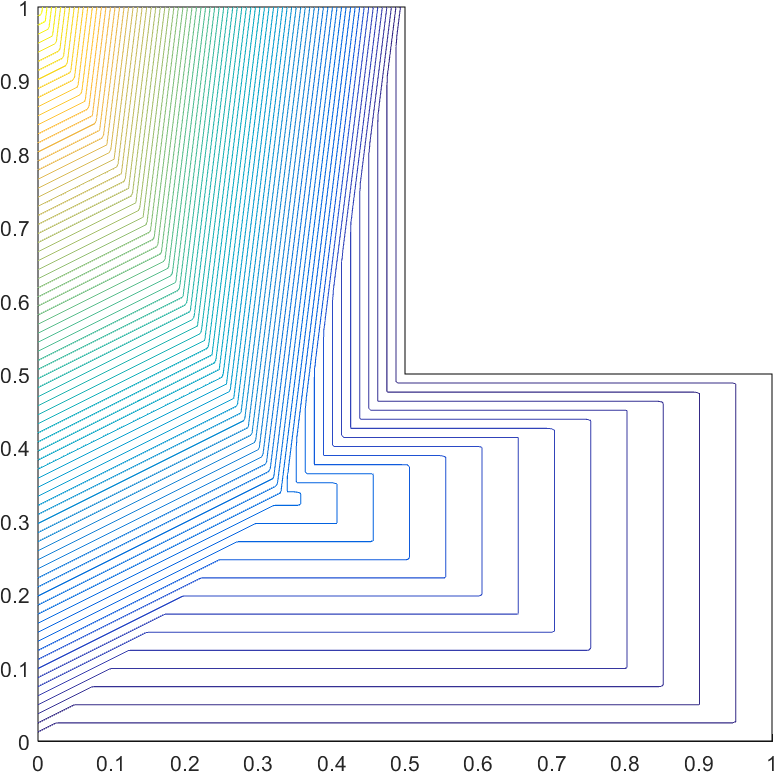
\includegraphics[width=0.85\columnwidth]{images/L-domain_PWLD1_contour_b6.png}\\
PWL\\ 
\column{0.333\textwidth}
\centering
{}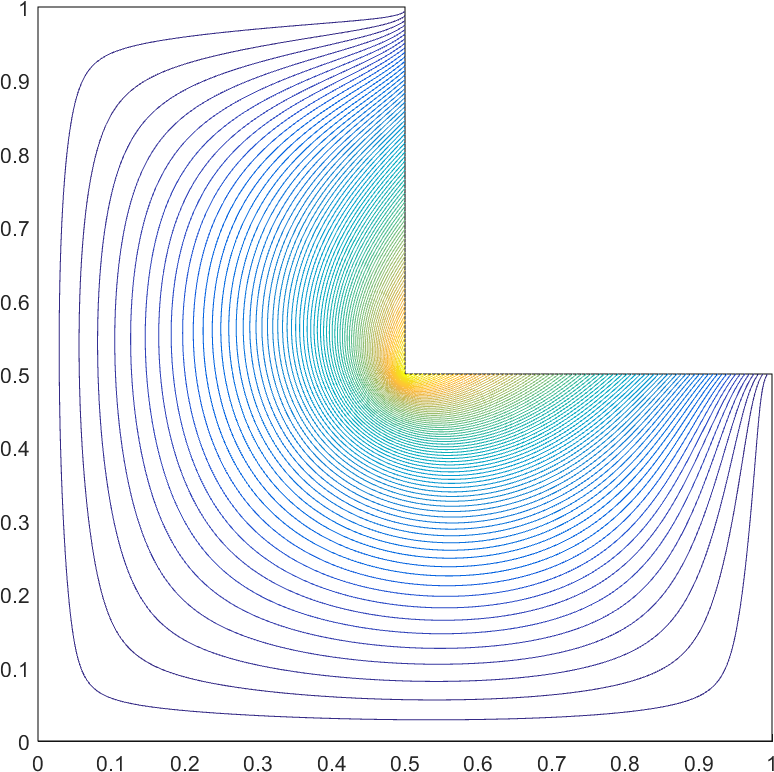
\includegraphics[width=0.85\columnwidth]{images/L-domain_MV1_contour_b4.png} \\
\vspace{3mm}
{}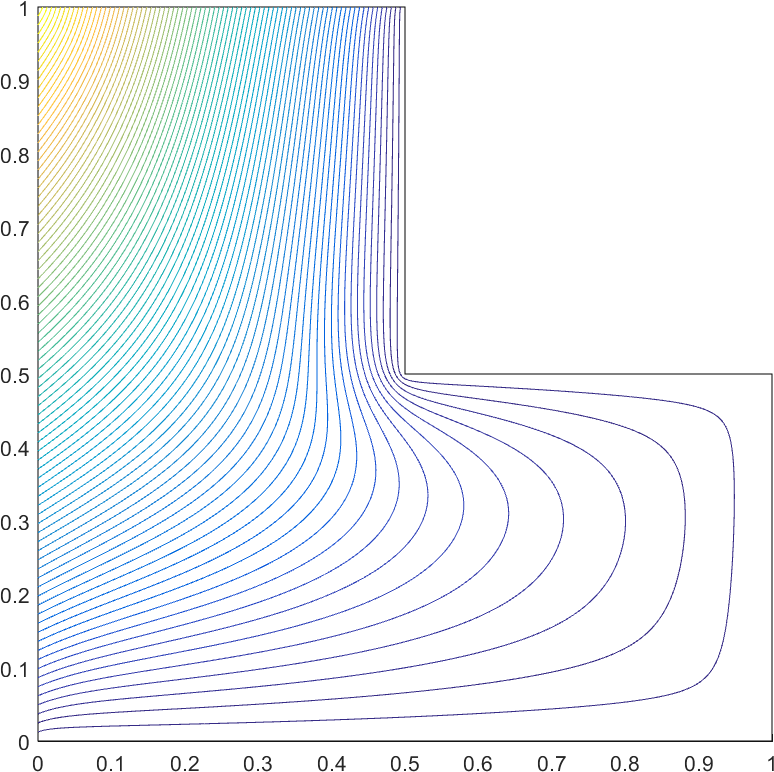
\includegraphics[width=0.85\columnwidth]{images/L-domain_MV1_contour_b6.png}\\
Mean Value
\column{0.333\textwidth}
\centering
{}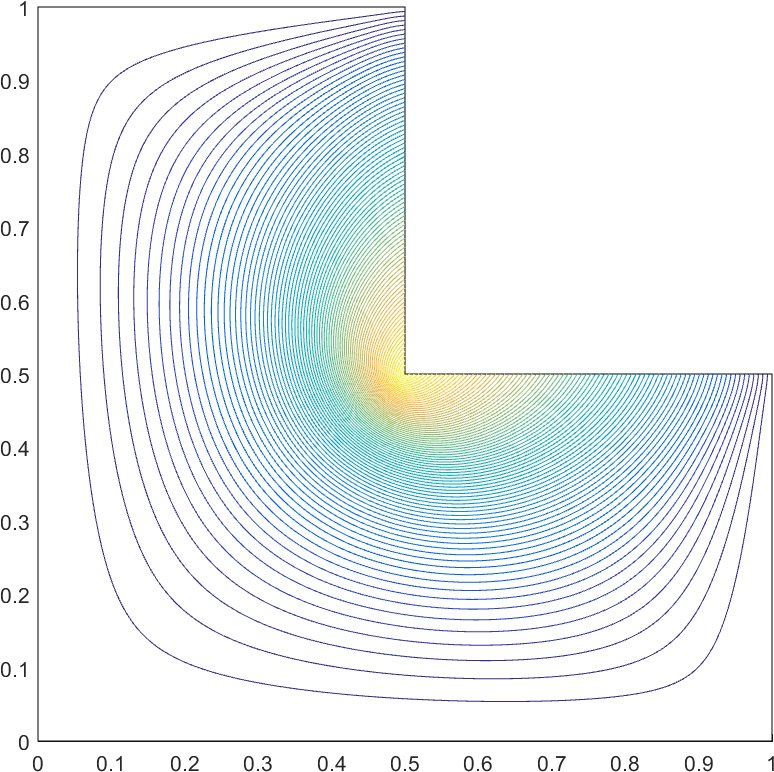
\includegraphics[width=0.85\columnwidth]{images/L-domain_MAXENT1_contour_b4.png} \\
\vspace{3mm}
{}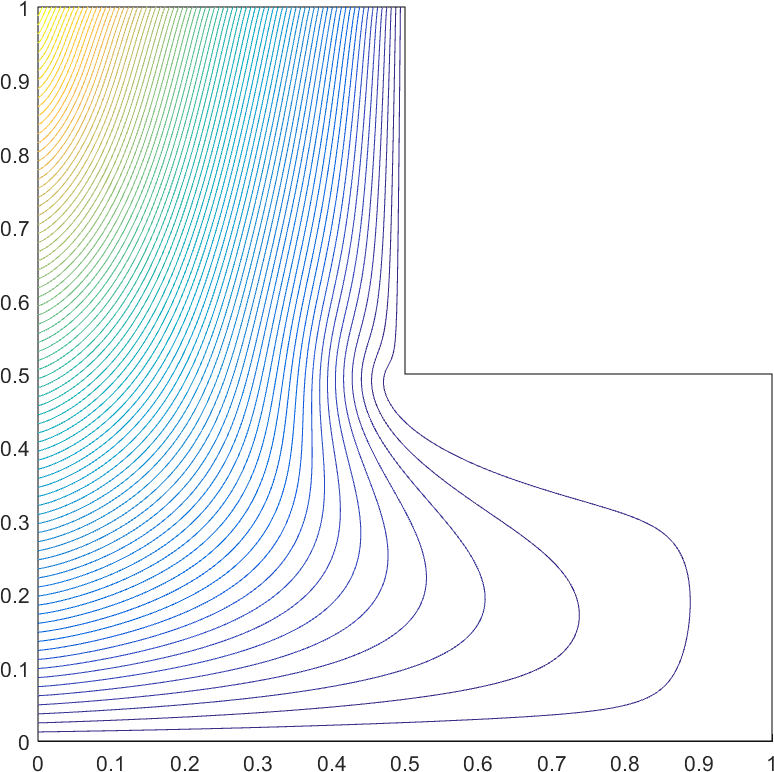
\includegraphics[width=0.85\columnwidth]{images/L-domain_MAXENT1_contour_b6.png} \\
Maximum Entropy
\end{columns}
}
\end{frame}
% --------------------------------------------
%%%%%%%%%%%%%%%%%%%
\subsection{Quadratic Basis Functions on Polygons}
%%%%%%%%%%%%%%%%%%%
% --------------------------------------------
\begin{frame}[t]\frametitle{Quadratic Serendipity Basis Functions on 2D Polygons}
\begin{block}{}
\begin{enumerate}
	\item <1-> Form the linear barycentric functions - \{$\lambda_i$\}
	\item <2-> Construct the pairwise products -  \{$\mu_{ab}$\}
	\item <3-> Eliminate the interior nodes to form a serendipity basis - \{$\xi_{ij}$\}
\end{enumerate}
\end{block}
\vspace{1cm}
\begin{columns}[c]
\column{0.28\textwidth}
\centering
\only<1-3>{
{}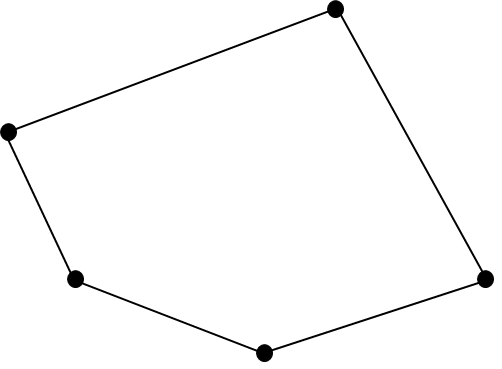
\includegraphics[width=0.9\columnwidth]{images/rand_linear.png} \\
\{$\lambda_i$\} \\
Linear
}
\column{0.08\textwidth}
\only<2-3>{
$\longrightarrow$
}
\column{0.28\textwidth}
\centering
\only<2-3>{
{}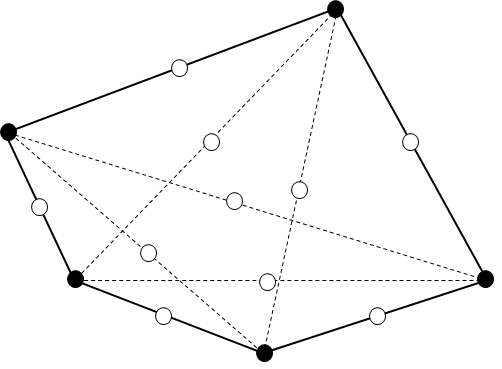
\includegraphics[width=0.9\columnwidth]{images/rand_quadratic.png} \\
\{$\mu_{ab}$\} \\
Quadratic
}
\column{0.08\textwidth}
\only<3>{
$\longrightarrow$
}
\column{0.28\textwidth}
\centering
\only<3>{
{}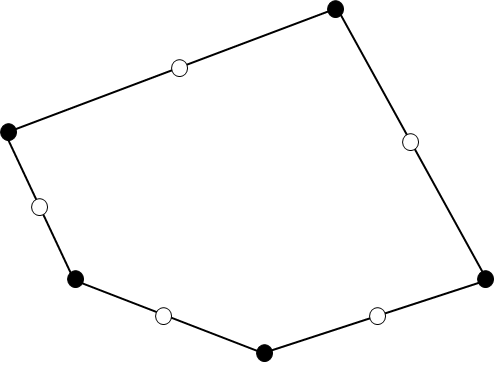
\includegraphics[width=0.9\columnwidth]{images/rand_serendipity.png} \\
\{$\xi_{ij}$\} \\
Serendipity
}
\end{columns}
\end{frame}
% --------------------------------------------
\begin{frame}[t]\frametitle{Pairwise products of the barycentric basis functions - $\mu_{ab} = \lambda_a \lambda_b$}
\only<1>{
\centering
{}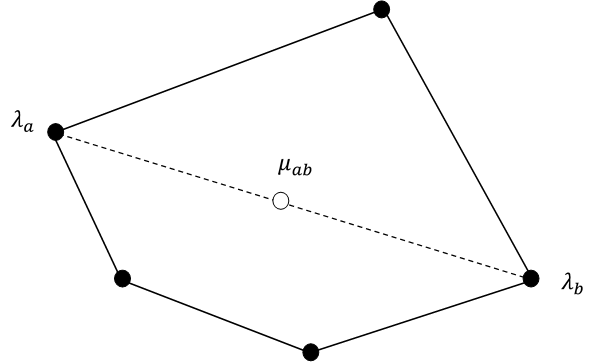
\includegraphics[width=0.75\columnwidth]{images/rand_quad_ab.png} 
}
\only<2>{
\begin{block}{Necessary Constraints}
\begin{columns}
\column{0.62\textwidth}
\begin{equation*}
\sum_{aa \in V} \mu_{aa} + \sum_{ab \in E \cup D} 2 \mu_{ab} = 1
\end{equation*}
\begin{equation*}
\sum_{aa \in V} \vec{x}_{aa} \mu_{aa} + \sum_{ab \in E \cup D} 2 \vec{x}_{ab} \mu_{ab} = \vec{x}
\end{equation*}
\begin{equation*}
\sum_{aa \in V} \vec{x}_{a} \vec{x}_{a}^T \mu_{aa} + \sum_{ab \in E \cup D} \left(  \vec{x}_{a} \vec{x}_{b}^T + \vec{x}_{b} \vec{x}_{a}^T  \right) \mu_{ab} = \vec{x} \vec{x}^{T}
\end{equation*}
\column{0.03\textwidth}
\column{0.35\textwidth}
{\small
$V$ - vertex nodes \\
$E$ - face midpoint nodes \\
$D$ - interior diagonal nodes \\ \vspace{3mm}
$V+E+D = n + n + \frac{n(n-3)}{2}$
}
\end{columns}
\end{block}
\begin{block}{Further Notation/Notes}
\begin{equation*}
\vec{x}_{ab} = \frac{\vec{x}_{a} + \vec{x}_{b}}{2}, \qquad \mu_{ab} = \lambda_a \lambda_b
\end{equation*}
\vspace{0.4cm}
\begin{equation*}
\mu^{K}_{ab}(\vec{r}) = 0, \qquad \left\{ ab \in D , \, \vec{r} \in \partial K  \right\}
\end{equation*}
\end{block}
}
\end{frame}
% --------------------------------------------
\begin{frame}[t]\frametitle{Eliminate interior nodes to form Serendipity basis}

\end{frame}
% --------------------------------------------
\begin{frame}[t]
\only<1>
{
\frametitle{Quadratic Basis Functions on the Unit Square}
\begin{columns}
\column{0.50\textwidth}
\centering
{}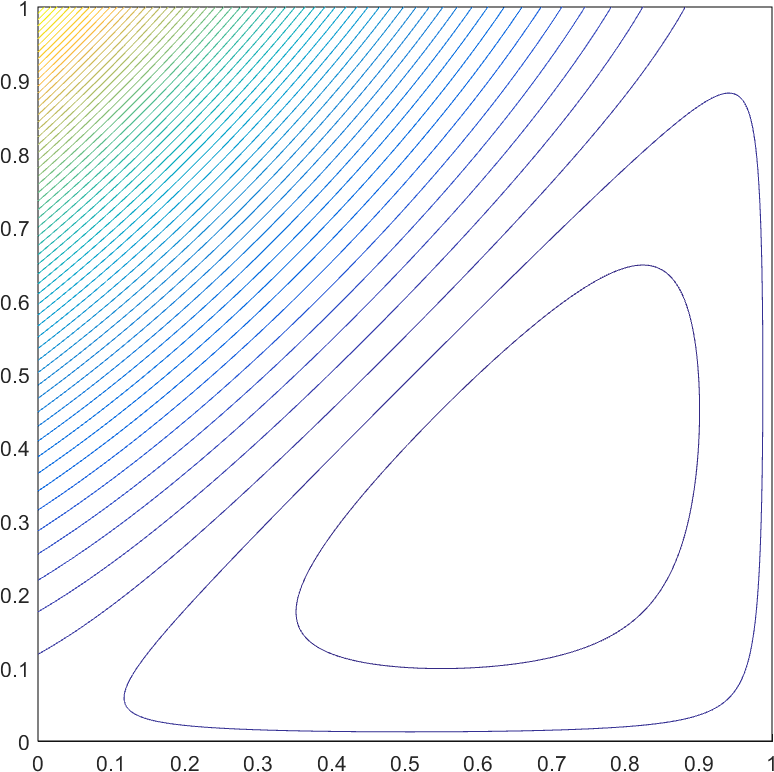
\includegraphics[width=0.55\columnwidth]{images/square_WACHSPRESS2_contour_b4.png} \\
Wachspress\\ \vspace{3mm}
{}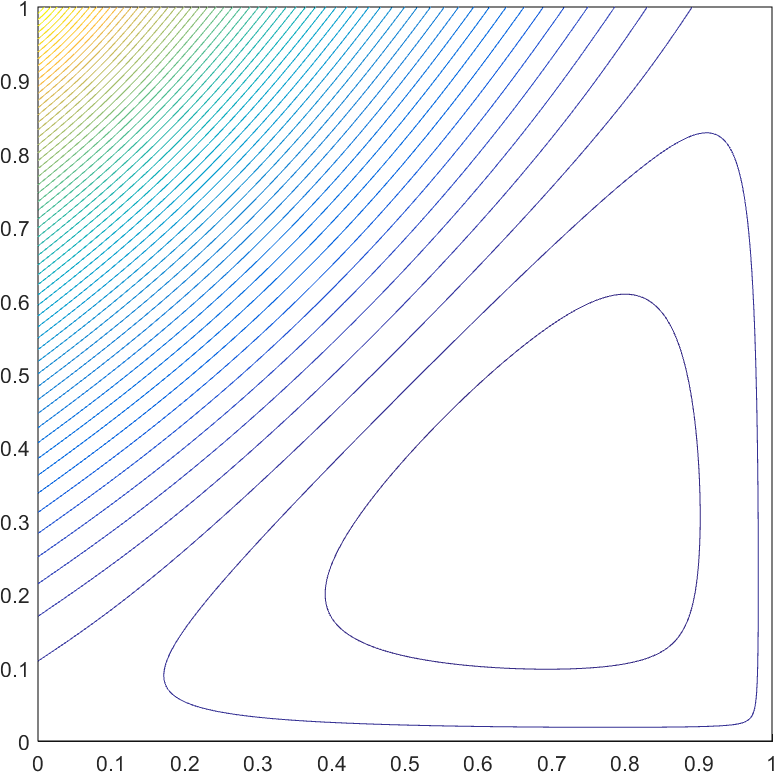
\includegraphics[width=0.55\columnwidth]{images/square_MV2_contour_b4.png} \\
Mean Value
\column{0.50\textwidth}
\centering
{}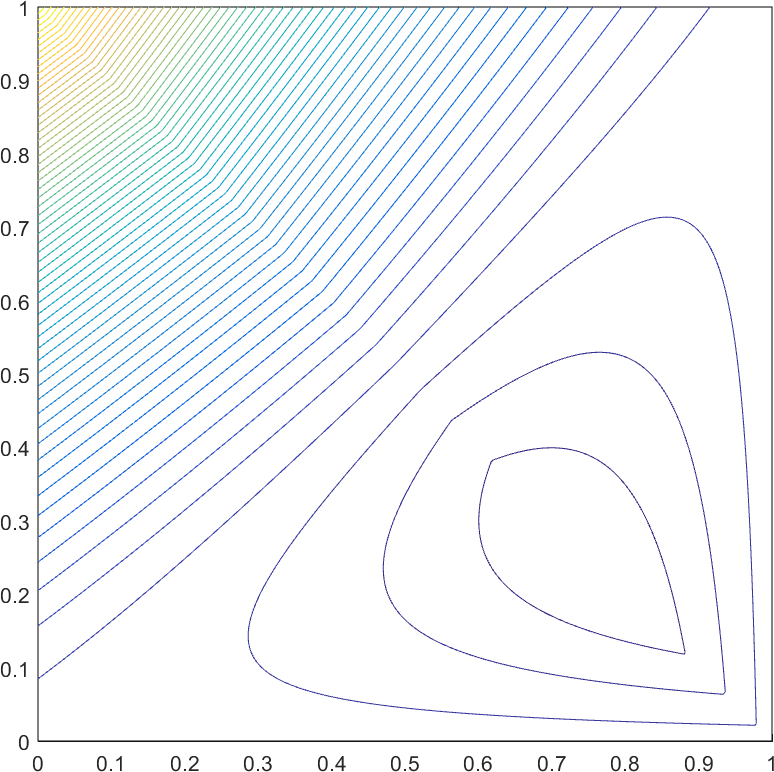
\includegraphics[width=0.55\columnwidth]{images/square_PWLD2_contour_b4.png} \\
PWL\\ \vspace{3mm}
{}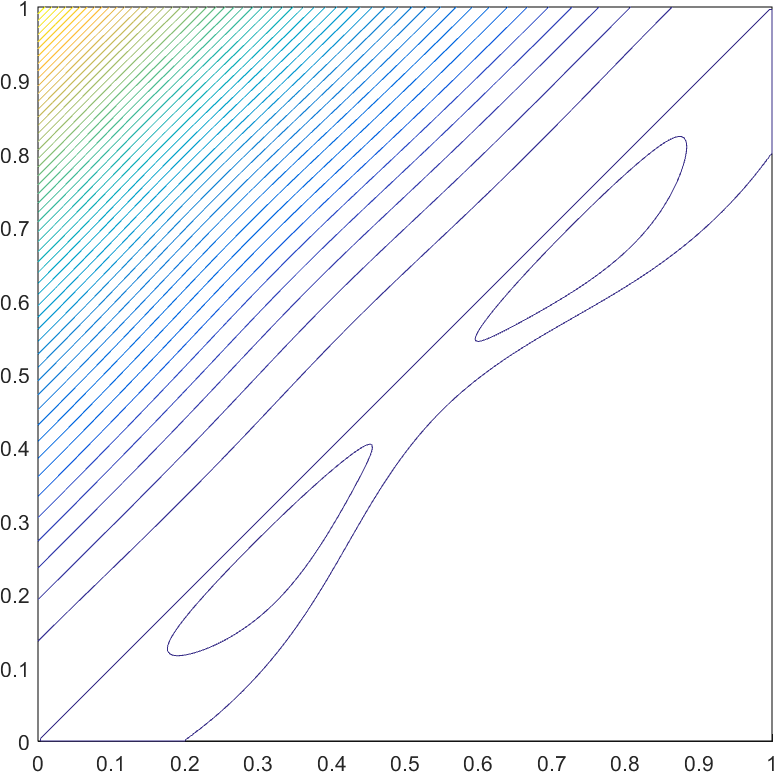
\includegraphics[width=0.55\columnwidth]{images/square_MAXENT2_contour_b4.png} \\
Maximum Entropy
\end{columns}
}
\only<2>
{
\frametitle{Quadratic Basis Functions on the Unit Square}
\begin{columns}
\column{0.50\textwidth}
\centering
{}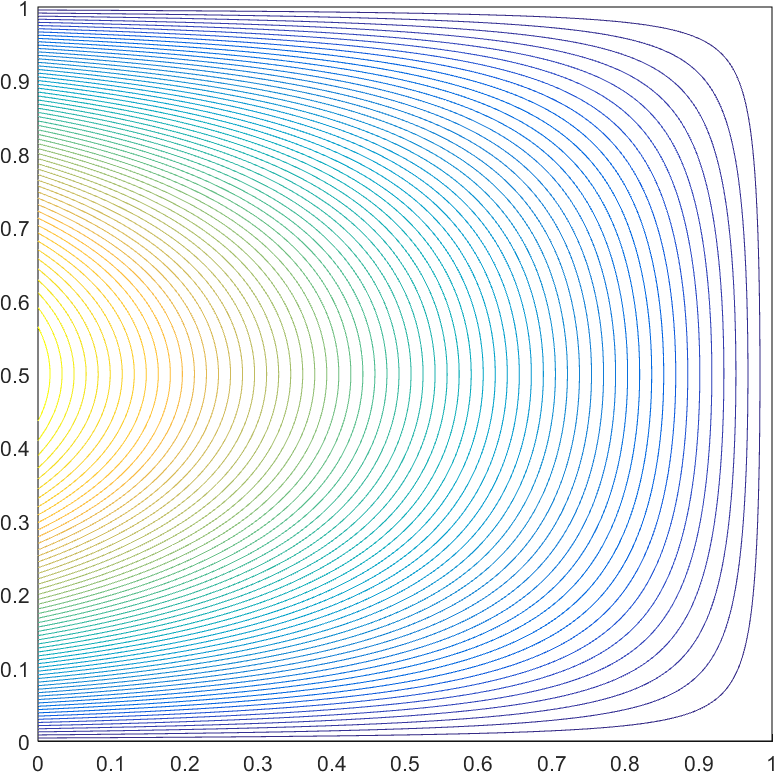
\includegraphics[width=0.55\columnwidth]{images/square_WACHSPRESS2_contour_b8.png} \\
Wachspress\\ \vspace{3mm}
{}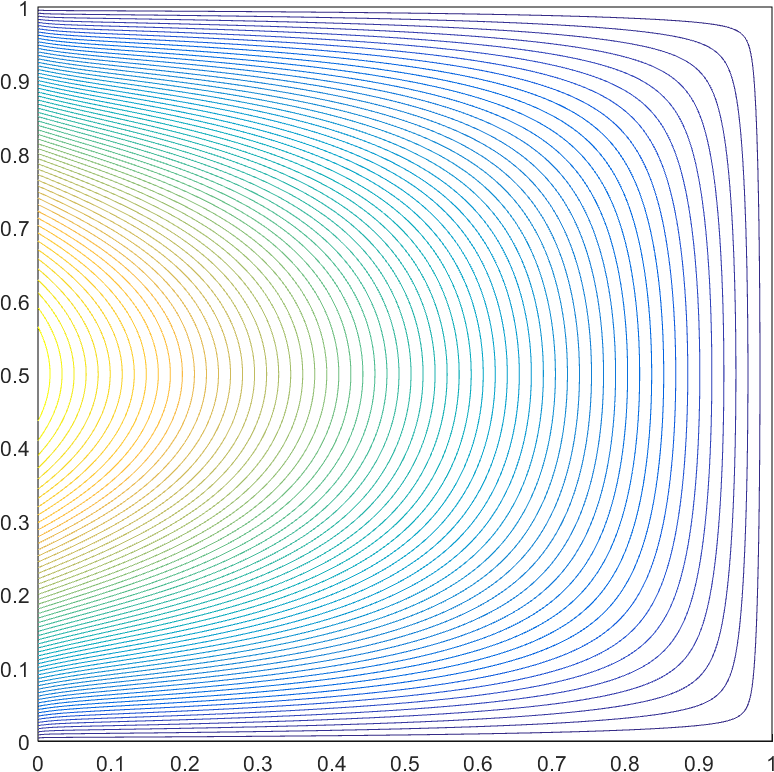
\includegraphics[width=0.55\columnwidth]{images/square_MV2_contour_b8.png} \\
Mean Value
\column{0.50\textwidth}
\centering
{}\includegraphics[width=0.55\columnwidth]{images/square_PWLD2_contour_b8.png} \\
PWL\\ \vspace{3mm}
{}\includegraphics[width=0.55\columnwidth]{images/square_MAXENT2_contour_b8.png} \\
Maximum Entropy
\end{columns}
}
\only<3>
{
\frametitle{Quadratic Basis Functions on the Degenerate Pentagon}
\begin{columns}
\column{0.333\textwidth}
\centering
{}\includegraphics[width=0.85\columnwidth]{images/deg_square_PWLD2_contour_b5.png} \\
\vspace{3mm}
{}\includegraphics[width=0.85\columnwidth]{images/deg_square_PWLD2_contour_b9.png} \\
PWL\\ 
\column{0.333\textwidth}
\centering
{}\includegraphics[width=0.85\columnwidth]{images/deg_square_MV2_contour_b5.png} \\
\vspace{3mm}
{}\includegraphics[width=0.85\columnwidth]{images/deg_square_MV2_contour_b9.png} \\
Mean Value
\column{0.333\textwidth}
\centering
{}\includegraphics[width=0.85\columnwidth]{images/deg_square_MAXENT2_contour_b5.png} \\
\vspace{3mm}
{}\includegraphics[width=0.85\columnwidth]{images/deg_square_MAXENT2_contour_b9.png} \\
Maximum Entropy
\end{columns}
}
\end{frame}
% --------------------------------------------
%%%%%%%%%%%%%%%%%%%
\subsection{Linear Basis Functions on Polyhedra}
%%%%%%%%%%%%%%%%%%%
% --------------------------------------------
\setbeamerfont{frametitle}{size=\large}
\begin{frame}[t]{Linear Basis Functions on 3D Polyhedra}
\begin{block}{Linear basis functions and convex polyhedra only for 3D}{\small
\begin{itemize}
\item The 2D quadratic serendipity formulation is more arduous in 3D
\item Intercell coupling is not straightforward for concave polyhedra
\item Focus on 3D PWL functions
\item Focus on 3D parallelepipeds and extruded convex polygons (convex prisms)
\end{itemize}}
\end{block}
\begin{block}{3D PWL basis functions}{\small
\begin{equation*}
b_i (\vec{x})  = t_i  (\vec{x})  + \sum_{f=1}^{F_i} \beta_f^i  t_f (\vec{x}) + \alpha_i t_c  (\vec{x}) 
\end{equation*}
}\end{block}
\begin{block}{}{\footnotesize
$t_i$ - standard 3D linear function for a tet $(i,i+1,f_c,K_c)$; 1 at vertex $i$, linearly decreases to 0 to the cell center, each adjoining face center, and each adjoining vertex\\ \vspace{0.5mm}
$t_c$ - 3D tent function; 1 at cell center, linearly decreases to 0 at all vertices and face centers \\ \vspace{0.5mm}
$t_f$ - face tent function; 1 at face center, linearly decreases to 0 at each face vertex and cell center\\ \vspace{0.5mm}
$\alpha_i = \frac{1}{N_V}$ - weight parameter for vertex $i$\\ \vspace{0.5mm}
$\beta_f^i = \frac{1}{N_f}$ - weight parameter for face $f$ touching vertex $i$
}\end{block}
\end{frame}
% --------------------------------------------
%%%%%%%%%%%%%%%%%%%
\subsection{Results}
%%%%%%%%%%%%%%%%%%%
% --------------------------------------------
\begin{frame}[t]\frametitle{Results Summary}
\begin{block}{}
\begin{enumerate}
\item Linear and quadratic basis functions capture the thick diffusion limit.
\item Linear basis functions capture exactly-linear transport solutions.
\item Quadratic basis functions capture exactly-quadratic transport solutions.
\item Convergence rate analysis using the Method of Manufactured Solutions. 
\item Convergence rate analysis bound by the solution regularity.
\end{enumerate}
\end{block}
\end{frame}
% --------------------------------------------
\begin{frame}[t]
\only<1>
{
\frametitle{Thick Diffusion Limit}
\begin{block}{Sufficient Basis Function Properties for Full Resolution}
\begin{itemize}
\item Locality of basis function integration on faces
\item Surface matching of basis functions across faces
\end{itemize}
\end{block}
\begin{block}{}

\end{block}
}
\only<2>
{
\frametitle{Thick Diffusion Limit}

}
\only<3>
{
\frametitle{Cartesian Mesh Convergence Rate}
\centering
{}\includegraphics[width=0.80\columnwidth]{images/DLConvergenceError_Cartesian.eps}
}
\only<4>
{
\frametitle{Polygonal Mesh Convergence Rate}
\centering
{}\includegraphics[width=0.80\columnwidth]{images/DLConvergenceError_SqPoly.eps}
}
\end{frame}
% --------------------------------------------
\begin{frame}[t]\frametitle{Exactly-Linear Transport Solutions}
\only<1>
{
\begin{block}{MMS Solution}
\begin{equation*}
\mu \frac{\partial \psi}{\partial x} + \eta \frac{\partial \psi}{\partial y} + \sigma_t \psi = Q(x,y, \mu, \eta)
\end{equation*}
\vspace{5mm}
\begin{equation*}
\begin{aligned}
\psi (x,y,\mu,\eta) &= ax + by + c \mu + d\eta + e\\
\phi (x,y) &= 2 \pi \left( ax + by  + e \right)
\end{aligned} 
\end{equation*}
\end{block}
\begin{block}{Forcing Function}
\begin{equation*}
Q(x,y,\mu,\eta) = a \mu + b \eta + \sigma_t \left(  c \mu + d \eta \right) + \sigma_t \left( ax +by + e   \right)
\end{equation*}
\vspace{3mm}
\begin{equation*}
\sigma_t = a = c = d = e = 1.0 \qquad b=1.5
\end{equation*}
\end{block}
}
\only<2>
{
\centering
\begin{columns}
\column{0.333\textwidth}
\centering
{}\includegraphics[width=0.95\columnwidth]{images/tri_MAXENT_k1.eps} \\
\vspace{3mm}
{}\includegraphics[width=0.95\columnwidth]{images/cart_MAXENT_k1.eps}
\column{0.333\textwidth}
\centering
{}\includegraphics[width=0.95\columnwidth]{images/shes_poly_MAXENT_k1.eps} \\
\vspace{3mm}
{}\includegraphics[width=0.95\columnwidth]{images/smooth_poly_MAXENT_k1.eps} 
\column{0.333\textwidth}
\centering
{}\includegraphics[width=0.95\columnwidth]{images/z_quad_MAXENT_k1.eps} \\
\vspace{3mm}
{}\includegraphics[width=0.95\columnwidth]{images/z_poly_MAXENT_k1.eps} 
\end{columns}
}
\end{frame}
% --------------------------------------------
\begin{frame}[t]\frametitle{Exactly-Quadratic Transport Solutions}
\only<1>
{


}

\end{frame}
% --------------------------------------------
\begin{frame}[t]
\only<1>
{
\frametitle{Convergence Rate Analysis by MMS}
{\small
\begin{block}{Sinusoid Solution}
\begin{equation*}
\begin{aligned}
\Psi_s (x,y) = &\sin(\nu  \frac{\pi x}{L_x}) \sin(\nu  \frac{\pi y}{L_y}) \\ 
\Phi_s (x,y) = 2 \pi &\sin(\nu  \frac{\pi x}{L_x}) \sin(\nu  \frac{\pi y}{L_y})
\end{aligned} 
\end{equation*}
\begin{itemize}
\item Cartesian, triangular and Voronoi polygon meshes
\item Wachspress, PWL, MV, and MAXENT
\end{itemize}
\end{block}
\begin{block}{Localized Gaussian Solution}
\begin{equation*}
\begin{aligned}
\Psi_g (x,y) = & \frac{x (L_x - x)}{L_x^2} \frac{y (L_y - y)}{L_y^2} \exp(-\frac{(x-x_0)^2 + (y-y_0)^2}{L_x L_y}) \\ 
\Phi_g (x,y) = 2 \pi &\frac{x (L_x - x)}{L_x^2} \frac{y (L_y - y)}{L_y^2} \exp(-\frac{(x-x_0)^2 + (y-y_0)^2}{L_x L_y})
\end{aligned} 
\end{equation*}
\begin{itemize}
\item Use spatial Adaptive Mesh Refinement (AMR)
\item PWL, MV, and MAXENT
\end{itemize}
\end{block}
}
}
\only<2>
{
\frametitle{Cartesian Sinusoid MMS Results}
\vspace{1.5cm}
\begin{columns}
\column{0.40\textwidth}
{}\includegraphics[width=0.8\columnwidth]{images/cart_mesh.jpg}
\column{0.60\textwidth}
{}\includegraphics[width=0.9\columnwidth]{images/TransMMS_Sine_cart_err.eps}
\end{columns}
}
\only<3>
{
\frametitle{Triangular Sinusoid MMS Results}
\vspace{1.5cm}
\begin{columns}
\column{0.40\textwidth}
{}\includegraphics[width=0.8\columnwidth]{images/tri_mesh.jpg}
\column{0.60\textwidth}
{}\includegraphics[width=0.9\columnwidth]{images/TransMMS_Sine_tri_err.eps}
\end{columns}
}
\only<4>
{
\frametitle{Polygonal Sinusoid MMS Results}
\vspace{1.5cm}
\begin{columns}
\column{0.40\textwidth}
{}\includegraphics[width=0.8\columnwidth]{images/PolyMesh_mesh.eps}
\column{0.60\textwidth}
{}\includegraphics[width=0.9\columnwidth]{images/TransMMS_Sine_poly_err.eps}
\end{columns}
}
\only<5>
{
\frametitle{\footnotesize Gaussian AMR - Linear ME cycle 15 (left) and quadratic ME cycle 08 (right)}
\begin{columns}
\column{0.50\textwidth}
\centering
{}\includegraphics[width=0.70\columnwidth]{images/ME1_cart_Irr=1_tol=0.2_cyc15_mesh.eps} \\
{}\includegraphics[width=0.70\columnwidth]{images/ME1_cart_Irr=1_tol=0.2_cyc15_sol.eps}
\column{0.50\textwidth}
\centering
{}\includegraphics[width=0.70\columnwidth]{images/ME2_cart_Irr=1_tol=0.1_cyc08_mesh.eps} \\
{}\includegraphics[width=0.70\columnwidth]{images/ME2_cart_Irr=1_tol=0.1_cyc08_sol.eps}
\end{columns}
}
\only<6>
{
\frametitle{Gaussian MMS Results - \tcr{PWL}}
\hspace*{1.25cm}
{}\includegraphics[width=0.75\columnwidth]{images/TransportMMS_Gauss2D_PWL_Err.eps}
}
\only<7>
{
\frametitle{Gaussian MMS Results - \tcr{Mean Value}}
\hspace*{1.25cm}
{}\includegraphics[width=0.75\columnwidth]{images/TransportMMS_Gauss2D_MV_Err.eps}
}
\only<8>
{
\frametitle{Gaussian MMS Results - \tcr{Maximum Entropy}}
\hspace*{1.25cm}
{}\includegraphics[width=0.75\columnwidth]{images/TransportMMS_Gauss2D_MAXENT_Err.eps}
}
\end{frame}
% --------------------------------------------
\begin{frame}[t]
\only<1>
{
\frametitle{Purely-Absorbing Material Problem}
\begin{block}{Solution Regularity Constraint}

\end{block}
\begin{block}{Problem Configuration}
\begin{enumerate}
\item Level-Symmetric $S_4$ quadrature
\end{enumerate}
\end{block}
\begin{block}{Geometry Configuration}
\begin{enumerate}
\item Unit square domain
\item Cartesian, Triangular, Polygonal, and Split-Polygonal Meshes
\end{enumerate}
\end{block}
}
\only<2>
{
\frametitle{Incident Flux Configuration}
\vspace{1cm}
\hspace*{2.75cm}
{}\includegraphics[width=0.45\textwidth]{images/PA_Shading.png}
}
\only<3>
{
\frametitle{Non-Aligned Meshes}
\vspace{0.75cm}
\hspace*{0.25cm}
{}\includegraphics[width=0.475\textwidth]{images/PAMesh_Cart.png} 
{}\includegraphics[width=0.475\textwidth]{images/PAMesh_Poly.png}
}
\only<4>
{
\frametitle{Aligned Meshes}
\vspace{0.75cm}
\hspace*{0.25cm}
{}\includegraphics[width=0.475\textwidth]{images/PAMesh_Tri.png} 
{}\includegraphics[width=0.475\textwidth]{images/PAMesh_SplitPoly.png}
}
\only<5>
{
\frametitle{Left-Face Incidence Solutions}
\vspace{0.75cm}
\hspace*{0.25cm}
{}\includegraphics[width=0.475\textwidth]{images/PALeftSol_Poly.png} 
{}\includegraphics[width=0.475\textwidth]{images/PALeftSol_SplitPoly.png}
}
\only<6>
{
\frametitle{Left-Face and Top-Face Incidence Solutions}
\vspace{0.75cm}
\hspace*{0.25cm}
{}\includegraphics[width=0.475\textwidth]{images/PALeftTopSol_Poly.png} 
{}\includegraphics[width=0.475\textwidth]{images/PALeftTopSol_SplitPoly.png}
}
\only<7>
{
\frametitle{Mesh-Aligned - Left-Face Incidence}
\vspace{1.00cm}
\begin{columns}[c]
\column{0.5\textwidth}
\centering
{}\includegraphics[width=\textwidth]{images/PAErr_Left_SplitPoly_sig1.eps} \\
$\sigma_t = 1$
\column{0.5\textwidth}
\centering
{}\includegraphics[width=\textwidth]{images/PAErr_Left_SplitPoly_sig50.eps} \\
$\sigma_t = 50$
\end{columns}
}
\only<8>
{
\frametitle{NOT Mesh-Aligned - Left-Face Incidence}
\vspace{1.00cm}
\begin{columns}[c]
\column{0.5\textwidth}
\centering
{}\includegraphics[width=\textwidth]{images/PAErr_Left_Poly_sig1.eps} \\
$\sigma_t = 1$
\column{0.5\textwidth}
\centering
{}\includegraphics[width=\textwidth]{images/PAErr_Left_Poly_sig50.eps} \\
$\sigma_t = 50$
\end{columns}
}
\only<9>
{
\frametitle{Mesh-Aligned - Left-Face and Top-Face Incidence}
\vspace{1.00cm}
\begin{columns}[c]
\column{0.5\textwidth}
\centering
{}\includegraphics[width=\textwidth]{images/PAErr_LeftTop_SplitPoly_sig1.eps} \\
$\sigma_t = 1$
\column{0.5\textwidth}
\centering
{}\includegraphics[width=\textwidth]{images/PAErr_LeftTop_SplitPoly_sig50.eps} \\
$\sigma_t = 50$
\end{columns}
}
\only<10>
{
\frametitle{NOT Mesh-Aligned -  Left-Face and Top-Face Incidence}
\vspace{1.00cm}
\begin{columns}[c]
\column{0.5\textwidth}
\centering
{}\includegraphics[width=\textwidth]{images/PAErr_LeftTop_Poly_sig1.eps} \\
$\sigma_t = 1$
\column{0.5\textwidth}
\centering
{}\includegraphics[width=\textwidth]{images/PAErr_LeftTop_Poly_sig50.eps} \\
$\sigma_t = 50$
\end{columns}
}
\end{frame}
% --------------------------------------------
\iffalse
%%%%%%%%%%%%%%%%%%%%%%%%%%%%%%%%%%%%%%%%%%%%%%%%%%%%%%%%%%%%%%%%%%%%%%%%%%%%%%%%%%%%%%%%%%%%%%
%%%%%%%%%%%%%%%%%%%%%%%%%%%%%%%%%%%%%%%%%%%%%%%%%%%%%%%%%%%%%%%%%%%%%%%%%%%%%%%%%%%%%%%%%%%%%%
\typeout{***********************************************************************************}
\typeout{MIP Section}
%%%%%%%%%%%%%%%%%%%%%%%%%%%%%%%%%%%%%%%%%%%%%%%%%%%%%%%%%%%%%%%%%%%%%%%%%%%%%%%%%%%%%%%%%%%%%%
% MIP SECTION
\section[MIP Form]{DFEM Discretization of the Diffusion Equation}
%%%%%%%%%%%%%%%%%%%
\subsection{}
%%%%%%%%%%%%%%%%%%%
% --------------------------------------------
\begin{frame}[t]\frametitle{Synthetic Acceleration}
\begin{block}{Transport sweep and iteration error}{\small
\begin{columns}
\column{0.60\textwidth}
\begin{equation*}
\begin{aligned}
{\bf L} \psi^{\tcr{(\ell+1/2)}} &= {\bf M\Sigma} \phi^{\tcb{(\ell)}} +{\bf Q} \\ \vspace{1mm}
{\bf L} \delta \psi^{\tcr{(\ell+1/2)}} &= {\bf M\Sigma} \delta \phi^{\tcr{(\ell+1/2)}} + \underbrace{{\bf M\Sigma} (\phi^{\tcr{(\ell+1/2)}}-\phi^{\tcb{(\ell)}})}_{{\bf R}^{\tcr{(\ell+1/2)}}} 
\end{aligned}
\end{equation*}
\column{0.40\textwidth}
\begin{equation*}
\begin{aligned}
\delta \psi^{\tcr{(\ell+1/2)}} &\equiv \psi - \psi^{\tcr{(\ell+1/2)}} \\
\delta \phi^{\tcr{(\ell+1/2)}} &\equiv {\bf D} \delta \psi^{\tcr{(\ell+1/2)}}
\end{aligned}
\end{equation*}
\end{columns}
}
\end{block}
\vspace{-1.5mm}
\begin{block}{Error approximation and update}{\small
If we could exactly solve for the error, then the solution could be obtained immediately:
\begin{equation*}
\phi^{(\ell+1)} = \phi^{\tcr{(\ell+1/2)}} + \delta \phi^{\tcr{(\ell+1/2)}}
\end{equation*}
However, this is just as difficult as the original transport problem. Instead, we estimate the error using low-order operators:
\begin{equation*}
\tilde{{\bf A}} \delta \phi^{\tcr{(\ell+1/2)}} = \tilde{{\bf R}}^{\tcr{(\ell+1/2)}}
\end{equation*}
$\tilde{{\bf A}}$ is a low-order diffusion operator.
}
\end{block}
\end{frame}
% --------------------------------------------
\begin{frame}[t]\frametitle{Various DSA Implementations}
\begin{block}{Historical DSA Work}
\begin{itemize}
	\item Kopp \& Lebedev - independently proposed method
	\item Gelbard and Hageman (G\&B) - efficient convergence on fine meshes
	\item Reed - showed that G\&B diverged for coarse meshes
	\item Alcouffe - consistency yields efficiency and robustness
\end{itemize}
\end{block}
\onslide<2->{
\begin{block}{Fully-consistent DSA schemes}
\begin{itemize}
	\item Larsen fully-consistent four step
	\item Fully-consistent DSA (FCDSA)
\end{itemize}
\end{block}
\begin{block}{Partially-consistent DSA schemes}
\begin{itemize}
	\item Modified four step (M4S)
	\item Waering-Larsen-Adams (WLA)
	\item Modified Interior Penalty DSA (MIP)
\end{itemize}
\end{block}
}
\end{frame}
% --------------------------------------------
%%%%%%%%%%%%%%%%%%%
\subsection{Symmetric Interior Penalty Method}
%%%%%%%%%%%%%%%%%%%
%---------------------------
\begin{frame}[t]\frametitle{Symmetric Interior Penalty (SIP) Form [1]}
\begin{block}{Bilinear Form}{\small
\begin{equation*}
\begin{aligned}
a( \Phi, b)  &= \Big<  D \vec{\nabla}  \Phi , \vec{\nabla} b  \Big>_{\mathcal{D}} + \Big<  \sigma   \Phi ,  b  \Big>_{\mathcal{D}}    \\
&+  \tcr{\Big\{ \kappa_e^{SIP} [\![   \Phi ]\!] , [\![  b ]\!]\Big\}_{E_h^i}} - \tcr{\Big\{  [\![   \Phi ]\!] , \{\!\{  D \partial_n b \}\!\}\Big\}_{E_h^i}} -\tcr{\Big\{ \{\!\{  D \partial_n  \Phi \}\!\} , [\![ b ]\!]\Big\}_{E_h^i}} \\
&+ \tcb{\Big\{ \kappa_e^{SIP}   \Phi ,   b \Big\}_{\partial \mathcal{D}^d}} - \tcb{\Big\{   \Phi  ,  D \partial_n b \Big\}_{\partial \mathcal{D}^d}} - \tcb{\Big\{   D \partial_n  \Phi ,   b \Big\}_{\partial \mathcal{D}^d}}  +  \tcb{\frac{1}{2} \Big\{    \Phi ,   b \Big\}_{\partial \mathcal{D}^r}}
\end{aligned}
\end{equation*} }
\end{block}
\begin{block}{Linear Form}{\small
\begin{align*}
\ell (b) = \Big<  q, b  \Big>_{\mathcal{D}}  - \tcb{\Big\{   J_{0}, b  \Big\}_{\partial \mathcal{D}^n}} +  \tcb{2 \Big\{   J_{inc}, b  \Big\}_{\partial \mathcal{D}^r}} \\ + \tcb{\Big\{ \kappa_e^{SIP}   \Phi_0 ,   b \Big\}_{\partial \mathcal{D}^d}} - \tcb{\Big\{   \Phi_0  ,  D \partial_n b \Big\}_{\partial \mathcal{D}^d} }
\end{align*} }
\end{block}
\begin{block}{}{\footnotesize
[1] D.N. Arnold. ``An interior penalty finite element method with discontinuous elements.'' {\em SIAM J. Numer. Anal.}, 19:742-760, (1982).
}\end{block}
\end{frame}
%---------------------------
\begin{frame}[t]\frametitle{SIP Penalty Coefficient}
\begin{block}{}{
	\begin{equation*}
		\kappa_e^{SIP} \equiv 
		\begin{cases}
		\frac{C_B}{2} \left(  \frac{D^+}{h^+} + \frac{D^-}{h^-}  \right) & , e \in E_h^i \\
		C_B \frac{D^-}{h^-}  & , e \in \partial \mathcal{D}
		\end{cases}
	\end{equation*}}
	\begin{equation*}
		C_B = c p (p+1)
	\end{equation*}
\end{block}
\begin{block}{}
$c$ - user defined constant ($c \geq 1$) \\
$p$ - polynomial order of the finite element basis ($1,2,3,...$) \\
$D^{(+/-)}$ - diffusion coefficient defined on the positive/negative side of a face\\
$h^{(+/-)}$ - orthogonal projection defined on the positive/negative side of a face
\end{block}
\begin{block}{}
	\begin{equation*}
		u^{\pm} = \lim_{s \rightarrow 0^{\pm}} u ({\bf r} + s {\bf n})
	\end{equation*}
\end{block}
\end{frame}
%---------------------------
\begin{frame}[t]
\frametitle{Orthogonal Projection}
\only<1>
{
\vspace{1cm}
{}\includegraphics[width=0.425\textwidth]{images/Orth_proj_square.png} \hfill
{}\includegraphics[width=0.425\textwidth]{images/Orth_proj_pentagon.png}
}
\only<2>
{
\begin{block}{2D Orthogonal Projections}
\begin{table}
\centering
\begin{tabular}{|c|c|c|c|c|}
	\hline
	Number of Vertices & 3 & 4 & $>4$ and even& $>4$ and odd \\
	\hline
	$h$ & $2 \frac{A_K}{L_f}$ & $\frac{A_K}{L_f}$ & $4 \frac{A_K}{P_K}$ & $2 \frac{A_K}{P_K} + \sqrt{\frac{2 A_K}{N_K \sin(\frac{2 \pi}{N_K})}}$ \\
	\hline
\end{tabular}
\end{table}
\vspace{3mm}
$N_K$ - \# of vertices for polygon $K$\\
$A_K$ - Area of polygon $K$\\
$L_f$  - Length of face $f$\\
$P_K$ - Perimeter for polygon $K$
\end{block}
\begin{block}{3D Orthogonal Projections}
\begin{table}
\centering
\begin{tabular}{|c|c|c|c|}
	\hline
	Number of Faces & 4 & 6 & otherwise \\
	\hline
	$h$ & $3 \frac{V_K}{A_f}$ & $\frac{V_K}{A_f}$ & $6 \frac{V_K}{SA_K}$  \\ [1ex]
	\hline
\end{tabular}
\end{table}
\vspace{3mm}
$V_K$  - Volume of polyhedron $K$\\
$A_f$   - Area of face $f$\\
$SA_K$ - Surface area of polyhedron $K$
\end{block}
}
\end{frame}
%---------------------------
%%%%%%%%%%%%%%%%%%%
\subsection{Modified Interior Penalty Method}
%%%%%%%%%%%%%%%%%%%
%---------------------------
\begin{frame}[t]\frametitle{Modified Interior Penalty (MIP) Form}

Recall the DSA equation:
\begin{equation*}
{\bf \tilde{A}} \tcr{\delta \phi}^{(\ell+1/2)} = \tilde{{\bf R}}^{(\ell+1/2)}
\end{equation*}

\begin{block}{Diffusion Form}{\footnotesize
\begin{gather*}
\Big<  D \vec{\nabla} \tcr{\delta \Phi} , \vec{\nabla} b  \Big>_{\mathcal{D}} 
+ \Big<  \sigma \tcr{\delta  \Phi} ,  b  \Big>_{\mathcal{D}}    \\
+ \Big\{ \kappa_e^{MIP} [\![ \tcr{\delta  \Phi} ]\!] , [\![  b ]\!]\Big\}_{E_h^i} 
- \Big\{  [\![  \tcr{\delta \Phi} ]\!] , \{\!\{  D \partial_n b \}\!\}\Big\}_{E_h^i} 
- \Big\{ \{\!\{  D \partial_n \tcr{\delta \Phi} \}\!\} , [\![ b ]\!]\Big\}_{E_h^i} \\
+ \Big\{ \kappa_e^{MIP} \tcr{\delta \Phi} ,   b \Big\}_{\partial \mathcal{D}^{vac}} -  \frac{1}{2} \Big\{  \tcr{\delta \Phi}  ,  D \partial_n b \Big\}_{\partial \mathcal{D}^{vac}} -  \frac{1}{2} \Big\{   D \partial_n \tcr{\delta \Phi} ,   b \Big\}_{\partial \mathcal{D}^{vac}}  \\
 = \Big<  R , b  \Big>_{\mathcal{D}}  +  \Big\{  \tcr{\delta J_{inc}}, b  \Big\}_{\partial \mathcal{D}^{ref}}
\end{gather*} }
\end{block}
	\begin{block}{MIP Penalty Term}{\footnotesize
		\begin{align*}
			\kappa_e^{MIP} = \max(\frac{1}{4},  \kappa_e^{SIP})
		\end{align*} }
	\end{block}
\end{frame}
%---------------------------
%%%%%%%%%%%%%%%%%%%
\subsection{Results}
%%%%%%%%%%%%%%%%%%%
% --------------------------------------------
\begin{frame}[t]\frametitle{MIP Results Summary}
\begin{block}{}
\begin{enumerate}
\item
\end{enumerate}
\end{block}
\end{frame}
% --------------------------------------------
\begin{frame}[t]
\only<1>
{
\frametitle{\small 2D Unit Square Fourier Results - linear (left) and quadratic (right) \tcr{Wachspress}}
\vspace{1cm}
\includegraphics[width=0.495\textwidth]{images/SI_MIP_quad_C=4_UWACHSPRESS1_LS.eps}
\includegraphics[width=0.495\textwidth]{images/SI_MIP_quad_C=4_UWACHSPRESS2_LS.eps}
}
\only<2>
{
\frametitle{\small 2D Unit Square Fourier Results - linear (left) and quadratic (right) \tcr{PWL}}
\vspace{1cm}
\includegraphics[width=0.495\textwidth]{images/SI_MIP_quad_C=4_PWLD1_LS.eps}
\includegraphics[width=0.495\textwidth]{images/SI_MIP_quad_C=4_UPWLD2_LS.eps}
}
\only<3>
{
\frametitle{\small 2D Unit Square Fourier Results - linear (left) and quadratic (right) \tcr{Mean Value}}
\vspace{1cm}
\includegraphics[width=0.495\textwidth]{images/SI_MIP_quad_C=4_UMV1_LS.eps}
\includegraphics[width=0.495\textwidth]{images/SI_MIP_quad_C=4_UMV2_LS.eps}
}
\only<4>
{
\frametitle{\small 2D Unit Square Fourier Results - linear (left) and quadratic (right) \tcr{Maximum Entropy}}
\vspace{1cm}
\includegraphics[width=0.495\textwidth]{images/SI_MIP_quad_C=4_MAXENT1_LS.eps}
\includegraphics[width=0.495\textwidth]{images/SI_MIP_quad_C=4_UMAXENT2_LS.eps}
}
\end{frame}
% --------------------------------------------
\begin{frame}[t]
\only<1>
{
\frametitle{Unit Cube PWL Fourier Analysis}
\vspace{1cm}
\begin{columns}
\column{0.5\textwidth}
\centering
\includegraphics[width=\textwidth]{images/SI_MIP_hex_C=1_PWLD_LS.eps}\\
$c=1$
\column{0.5\textwidth}
\centering
\includegraphics[width=\textwidth]{images/SI_MIP_hex_C=4_PWLD_LS.eps}\\
$c=4$
\end{columns}
}
\only<2>
{
\frametitle{3D PWL Fourier Analysis - Aspect Ratios}
\vspace{1cm}
\begin{columns}
\column{0.5\textwidth}
\centering
\includegraphics[width=\textwidth]{images/SI_MIP_hex_PWLD1_AR1.eps}\\
$c=1,$ $S_8$
\column{0.5\textwidth}
\centering
\includegraphics[width=\textwidth]{images/SI_MIP_hex_PWLD1_AR4.eps}\\
$c=4,$ $S_8$
\end{columns}
}
\only<3>
{
\frametitle{Numerical 3D PWL Results}
\vspace{1cm}
\begin{columns}
\column{0.5\textwidth}
\centering
\includegraphics[width=\textwidth]{images/SI_MIP_hex_C=1_PWLD_LS_wNSR.eps}\\
$c=1$
\column{0.5\textwidth}
\centering
\includegraphics[width=\textwidth]{images/SI_MIP_hex_C=4_PWLD_LS_wNSR.eps}\\
$c=4$
\end{columns}
}
\end{frame}
% --------------------------------------------
\begin{frame}[t]
\only<1>
{
\frametitle{MIP Scaling Results}

}
\only<2>
{
\frametitle{512 cells/processor and 16 angles/octant}
\centering
\includegraphics[width=\textwidth]{images/A128.eps}
}
\only<3>
{
\frametitle{4096 cells/processor and 256 angles/octant}
\centering
\includegraphics[width=\textwidth]{images/A2048.eps}
}
\only<4>
{
\frametitle{DSA Timing Fraction - 512 cells/processor}
\centering
\includegraphics[width=\textwidth]{images/C512.eps}
}
\only<5>
{
\frametitle{DSA Timing Fraction - 4096 cells/processor}
\centering
\includegraphics[width=\textwidth]{images/C4096.eps}
}
\end{frame}
% --------------------------------------------
%%%%%%%%%%%%%%%%%%%%%%%%%%%%%%%%%%%%%%%%%%%%%%%%%%%%%%%%%%%%%%%%%%%%%%%%%%%%%%%%%%%%%%%%%%%%%%
%%%%%%%%%%%%%%%%%%%%%%%%%%%%%%%%%%%%%%%%%%%%%%%%%%%%%%%%%%%%%%%%%%%%%%%%%%%%%%%%%%%%%%%%%%%%%%
\typeout{***********************************************************************************}
\typeout{Upscatter Section}
%%%%%%%%%%%%%%%%%%%%%%%%%%%%%%%%%%%%%%%%%%%%%%%%%%%%%%%%%%%%%%%%%%%%%%%%%%%%%%%%%%%%%%%%%%%%%%
% UPSCATTERING SECTION
\section[Upscattering Acceleration]{Thermal Neutron Upscattering Acceleration}
%%%%%%%%%%%%%%%%%%%
\subsection{Overview of Methods}
%%%%%%%%%%%%%%%%%%%
% --------------------------------------------
\begin{frame}[t]\frametitle{Need for Upscatter Acceleration}
\begin{columns}
\column{0.65\textwidth}
\begin{block}{Slow Convergence Rates}
\begin{itemize}
\item
\item
\item
\end{itemize}
\end{block}
\column{0.35\textwidth}
\centering
\includegraphics[width=0.9\textwidth]{images/Sparsity_Graphite.eps} \\
\includegraphics[width=0.9\textwidth]{images/Sparsity_HDPE.eps}
\end{columns}
\end{frame}
% --------------------------------------------
\begin{frame}[t]\frametitle{Overview of Methods}
\begin{block}{Gauss-Seidel in Energy}

\end{block}
\begin{block}{Jacobi in Energy}

\end{block}
\end{frame}
%---------------------------
\begin{frame}[t]\frametitle{Three two-grid-like acceleration methodologies (implemented in PDT)}{\footnotesize
\vspace{-2.5mm}
\begin{block}{Standard Two-Grid Acceleration (TG) - Morel 1993}
\begin{itemize}
\item Gauss Seidel in energy - converging the within-group inner iterations
\end{itemize}
\begin{equation*}
{\bf L_{gg}} \psi_g^{(k+1)} = {\bf M} \sum_{g'=1}^{\tcb{g}} {\bf \Sigma}_{g g'} \phi_{g'}^{(k+1)} + {\bf M} \sum_{g'=\tcr{g+1}}^G {\bf \Sigma}_{g g'} \phi_{g'}^{(k)} + {\bf Q}_g
\end{equation*}
\end{block}
\vspace{-2.5mm}
\begin{block}{Modified Two-Grid Acceleration (MTG)}
\begin{itemize}
\item Do NOT converge the inner iterations
\begin{equation*}
{\bf L_{gg}} \psi_g^{(k+1)} = {\bf M} \sum_{g'=1}^{\tcm{g-1}} {\bf \Sigma}_{g g'} \phi_{g'}^{(k+1)} + {\bf M} \sum_{g'=\tcb{g}}^G {\bf \Sigma}_{g g'} \phi_{g'}^{(k)} + {\bf Q}_g
\end{equation*}
\end{itemize}
\end{block}
\vspace{-2.5mm}
\begin{block}{Mulitgroup Jacobi Acceleration (MJA)}
\begin{itemize}
\item Jacobi iterations in energy for some set of energy groups
\end{itemize}
\begin{equation*}
{\bf L_{gg}} \psi_g^{(k+1)} = {\bf M} \sum_{g'=1}^G {\bf \Sigma}_{g g'} \phi_{g'}^{(k)} + {\bf Q}_g
\end{equation*}
\end{block}
\vspace{-2.5mm}
\begin{block}{Acceleration Step}
\begin{itemize}
\item Each of these methods uses a 1-Group energy-collapsed acceleration step.
\end{itemize}
\end{block}
}
\end{frame}
%---------------------------
\begin{frame}[t]\frametitle{1-group Energy-Collapsed Diffusion Equation}
\vspace{-3mm}
\begin{block}{1G Correction System}{\small
\begin{itemize}
\item Factorize the error: $\delta \Phi_{g}^{(k+1/2)} = \tcr{\xi_g} \tcb{\epsilon^{(k+1/2)}}$
\item MG Solution Update:  $ \Phi_{g}^{(k+1)} =  \Phi_{g}^{(k+1/2)} + \tcr{\xi_g} \tcb{\epsilon^{(k+1/2)}}, \qquad \sum\displaylimits_{g=1}^{G} \tcr{\xi_g} = 1 $ 
\end{itemize}
\vspace{4mm}
\begin{equation*}
-\vec{\nabla} \cdot \Big< D \Big> \vec{\nabla} \tcb{\epsilon} + \Big< \sigma \Big> \tcb{\epsilon} = \Big< R \Big>
\end{equation*}
}\end{block}
\begin{block}{Spectral Distribution}{\small
\begin{columns}
\column{0.35\textwidth}
TG Acceleration:  \\ \vspace{3mm}
MTG Acceleration:  \\ \vspace{3mm}
MG Jacobi Acceleration:  \\
\column{0.63\textwidth}
$\left(  {\bf \Sigma_t} - {\bf S_{L}} - {\bf S_{D}} \right)^{-1} {\bf S_{U}} {\bf \tcr{\xi}} = \rho {\bf \tcr{\xi}}$ \\ \vspace{3mm}
$\left(  {\bf \Sigma_t} - {\bf S_{L}}  \right)^{-1} \left( {\bf S_{D}} + {\bf S_{U}} \right) {\bf \tcr{\xi}} = \rho {\bf \tcr{\xi}}$ \\ \vspace{3mm}
${\bf \Sigma_t}^{-1} \left( {\bf S_L} + {\bf S_D} +{\bf S_U} \right) {\bf \tcr{\xi}} = \rho {\bf \tcr{\xi}}$ \\
\end{columns}
}\end{block}
\end{frame}
% --------------------------------------------
%%%%%%%%%%%%%%%%%%%
\subsection{IM1 Results}
%%%%%%%%%%%%%%%%%%%
% --------------------------------------------
\begin{frame}[t]\frametitle{IM1 Problem}
\begin{block}{Iterative Procedures}
\begin{itemize}
	\item Brick grids
	\item 99 energy groups - 42 fast and 57 thermal
	\item Fast groups organized into 11 group sets to maximize downscatter
	\item Gauss-Seidel iterations (TG and MTG)
	\begin{itemize}
		\item Outer iterations march through thermal groups 1 at a time
		\item No thermal group parallelization
		\item Acceleration after each outer iteration
	\end{itemize}
	\item Jacobi iterations (MG Jacobi)
	\begin{itemize}
		\item All thermal groups in 1 group set
		\item No outer iterations (no iterative upscattering)
		\item Concurrent sweeping of all thermal groups
		\item Acceleration after each sweep of thermal group set
	\end{itemize}
\end{itemize}
\end{block}
\end{frame}
% --------------------------------------------
\begin{frame}[t]
\frametitle{IM1 Two-Grid Spectral Shapes}
\hspace*{1.1cm}
\includegraphics[width=0.75\textwidth]{images/IM1_EC_TG.eps}
\end{frame}
% --------------------------------------------
\begin{frame}[t]\frametitle{Infinite Medium Fourier Results}{\small
\vspace{0.85cm}
\begin{table}
\centering
\def\arraystretch{1.2}
\begin{tabular}{|c||c|c||c|c||c|c|c|}
\hline
Material  & U. TG & A. TG & U. MTG & A. MTG & U. MJA & A. MJA & A. MJIA \\ \hline
\tcr{Graphite} & \tcr{0.9883}&\tcb{0.4084}&\tcr{0.9993}&\tcr{0.9604}&\tcr{0.9993}&\tcr{0.9613}&\tcm{0.6462}\\
\tcr{HDPE} &\tcr{0.8916}&\tcb{0.4343}&\tcr{0.9918}&\tcr{0.7527}&\tcr{0.9943}&\tcr{0.8015}&\tcm{0.6631}\\
B-HDPE &0.0258&0.0177&0.1331&0.1221&0.1336&0.1223&0.0639 \\
Wood & 0.9820&0.2101&0.9840&0.3836&0.9915&0.5326&0.4684 \\
AmBe  &0.4835&0.2724&0.5646&0.5554&0.7068&0.5596&0.4947 \\
Steel  & 0.6989&0.5809&0.9243&0.9215&0.9255&0.9215&0.7547\\
Boral  & 0.0023&0.0016&0.0782&0.0602&0.0782&0.0602&0.0039 \\
BF3   & 0.0008&0.0006&0.0351&0.0266&0.0351&0.0266&0.0086 \\
Air     &0.7580&0.5282&0.8121&0.7828&0.8845&0.7896&0.7166\\
\hline
\end{tabular}
\end{table}
}\end{frame}
% --------------------------------------------
\begin{frame}[t]
\only<1>
{
\frametitle{\small Graphite Two-Grid Flat Mode Eigenvalues}
\hspace*{1.1cm}
\includegraphics[width=0.75\textwidth]{images/IM1_Graph_FA_TG.eps}
}
\only<2>
{
\frametitle{\small Graphite Modified Two-Grid Flat Mode Eigenvalues}
\hspace*{1.1cm}
\includegraphics[width=0.75\textwidth]{images/IM1_Graph_FA_MTG.eps}
}
\only<3>
{
\frametitle{\small Graphite Multigroup Jacobi Acceleration Flat Mode Eigenvalues}
\hspace*{1.1cm}
\includegraphics[width=0.75\textwidth]{images/IM1_Graph_FA_MJA.eps}
}
\only<4>
{
\frametitle{\small Graphite Multigroup Jacobi with Inner Acceleration Flat Mode Eigenvalues}
\hspace*{1.1cm}
\includegraphics[width=0.75\textwidth]{images/IM1_Graph_FA_MJIA.eps}
}
\end{frame}
% --------------------------------------------
\begin{frame}[t]\frametitle{2D Variant Results}{\footnotesize
\only<1>
{
\hspace*{1.75cm}
{}\includegraphics[width=0.60\textwidth]{images/2D_IM1_Variant_Layout.png}
}
\only<2>
{
\begin{block}{Two-Grid Results - $10^{-7}$ inner tolerance}
\begin{table}
\begin{tabular}{|c|c|c|c|c|}
\hline
Problem & Outer Iter. & Inner Iter. & 1-Group Sweeps & Solve Time (min)  \\
\hline \hline
\tcr{SI} & \tcr{361} & \tcr{185,422} &\tcr{185,422}  &  \tcr{486.50} \\ \hline
SI+DSA & 55 & 35,699 & 35,699 &  96.48 \\ \hline
GMRES & 38 & 41,575 & 41,575 &  128.63 \\ \hline
GMRES+DSA & 14 & 19,053 & 19,053  & 57.92  \\ \hline
\end{tabular}
\end{table}
\end{block}
\vspace{-3mm}
\begin{block}{Modified Two-Grid Results}
\begin{table}
\begin{tabular}{|c|c|c|c|c|}
\hline
Problem & Outer Iter. & Inner Iter. & 1-Group Sweeps & Solve Time (min)  \\
\hline \hline
\tcr{SI} & \tcr{536} & \tcr{77,632} & \tcr{77,632} & \tcr{275.83}  \\ \hline
SI+DSA & 73 & 10,846 & 10,846 &  40.60 \\ \hline
GMRES & 78 & 4,845 & 4,845 &  25.82 \\ \hline
GMRES+DSA & 26 & 1,881 & 1,881 & 11.09  \\ \hline
\end{tabular}
\end{table}
\end{block}
\vspace{-3mm}
\begin{block}{Multigroup Richardson Results}
\begin{table}
\begin{tabular}{|c|c|c|c|c|}
\hline
Problem & Outer Iter. & Inner Iter. & 1-Group Sweeps & Solve Time (min)  \\
\hline \hline
\tcr{SI} & \tcr{1} & \tcr{1,734} & \tcr{98,838} &  \tcr{111.07} \\ \hline
SI+DSA & 1 & 157 & 8,949 &  15.49 \\ \hline
GMRES & 1 & 118 & 6,726 &  8.65 \\ \hline
\tcb{GMRES+DSA} &  \tcb{1}& \tcb{35} & \tcb{1,995} &  \tcb{4.16} \\ \hline
\end{tabular}
\end{table}
\end{block}
}
}
\end{frame}
% --------------------------------------------
\begin{frame}[t]\frametitle{3D IM1 Results}{\footnotesize
\vspace{-2mm}
\begin{block}{Two-Grid Results}
\begin{table}
\begin{tabular}{|c|c|c|c|}
\hline
Problem & Outer Iter.  & 1-Group Sweeps & Solve Time (hr)  \\
\hline \hline
SI & - & -  & -  \\ \hline
SI+DSA & -  & - & -  \\ \hline
GMRES & -  & - & - \\ \hline
\tcr{GMRES+DSA} & \tcr{14} &  \tcr{11,104}  &  \tcr{$32.5^*$}  \\ \hline
\end{tabular}
\end{table}
\end{block}
\vspace{-2mm}
\begin{block}{Modified Two-Grid Results}
\begin{table}
\begin{tabular}{|c|c|c|c|}
\hline
Problem & Outer Iter.  & 1-Group Sweeps & Solve Time (hr)  \\
\hline \hline
SI & - &  - & -  \\ \hline
SI+DSA & -  & - & -  \\ \hline
\tcr{GMRES} & \tcr{81}  & \tcr{4,617 }& \tcr{$14.2^*$} \\ \hline
GMRES+DSA & 34 &  1,938  &  4.82  \\ \hline
\end{tabular}
\end{table}
\end{block}
\vspace{-2mm}
\begin{block}{Multigroup Richardson Results}
\begin{table}
\begin{tabular}{|c|c|c|c|}
\hline
Problem & Outer Iter. & 1-Group Sweeps & Solve Time (hr)  \\
\hline \hline
SI &  - & - & -  \\ \hline
SI+DSA & 256 &  14,592 & 11.2 \\ \hline
\tcm{GMRES} & \tcm{120} & \tcm{6,840} & \tcm{4.93} \\ \hline
\tcb{GMRES+DSA} & \tcb{31}& \tcb{1,767} & \tcb{1.76} \\ \hline
\end{tabular}
\end{table}
\end{block}
}
\end{frame}
% --------------------------------------------
%%%%%%%%%%%%%%%%%%%%%%%%%%%%%%%%%%%%%%%%%%%%%%%%%%%%%%%%%%%%%%%%%%%%%%%%%%%%%%%%%%%%%%%%%%%%%%
%%%%%%%%%%%%%%%%%%%%%%%%%%%%%%%%%%%%%%%%%%%%%%%%%%%%%%%%%%%%%%%%%%%%%%%%%%%%%%%%%%%%%%%%%%%%%%
\typeout{***********************************************************************************}
\typeout{Conclusions}
%%%%%%%%%%%%%%%%%%%%%%%%%%%%%%%%%%%%%%%%%%%%%%%%%%%%%%%%%%%%%%%%%%%%%%%%%%%%%%%%%%%%%%%%%%%%%%
% CONCLUSIONS SECTION
\section{Conclusions and Open Items}
\subsection{}
% --------------------------------------------
\begin{frame}[t]\frametitle{Conclusions}
\begin{block}{POLYFEM Conclusions}
\begin{enumerate}
\item
\item
\item
\item
\end{enumerate}
\end{block}
\begin{block}{DSA Conclusions}
\begin{enumerate}
\item
\item
\item
\item
\end{enumerate}
\end{block}
\end{frame}
% --------------------------------------------
\begin{frame}[t]\frametitle{Open Items}
\begin{block}{POLYFEM Open Items}
\begin{enumerate}
\item Quadratic serendipity basis functions on 3D polyhedra
\item Higher-order 2D serendipity polygonal basis functions
\item Alternative integration schemes on polygons
\end{enumerate}
\end{block}
\begin{block}{DSA Open Items}
\begin{enumerate}
\item Numerical verification of the MJIA method
\item Mixed-mode parallelism with DSA preconditioning
\end{enumerate}
\end{block}
\end{frame}
% --------------------------------------------

%%%%%%%%%%%%%%%%%%%%%%%%%%%%%%%%%%%%%%%%%%%%%%%%%%%%%%%%%%%%%%%%%%%%%%%%%%%%%%%%%%%%%%%%%%%%%
\typeout{***********************************************************************************}
\typeout{We have reached the end}

\begin{frame}[plain]
   \frametitle{Thank you!}

\vspace{25mm}

\begin{columns}[b]

\column{0.7\textwidth}

\centering

{\Large Questions?}

\vspace{9mm}
\footnotesize
A special acknowledgment to the Department of Energy Rickover Fellowship Program in Nuclear Engineering, which provides strong support to its fellows and their professional development.

\end{columns}

\vspace{10mm}

\begin{columns}[b]

\column{0.5\textwidth}
\centering
{}\includegraphics[width=0.35\figwidth]{images/DOE_logo.png}\\

\column{0.5\textwidth}
\centering
{}\includegraphics[width=0.70\figwidth]{images/tamu_engineering.png}\\

\end{columns}

\end{frame}

%%%%%%%%%%%%%%%%%%%%%%%%%%%%%%%%%%%%%%%%%%%%%%%%%%%%%%%%%%%%%%%%%%%%%%%%%%%%%%%%%%%%%%%%%%%

\fi



\backupbegin
\appendix

%%%%%%%%%%%%%%%%%%%%%%%%%%%%%%%%%%%%%%%%%%%%%%%%%%%%%%%%%%%%%%%%%%%%%%%%%%%%%%%%%%%%%%%%%%%%
%%%%%%%%%%%%%%%%%%%%%%%%%%%%%%%%%%%%%%%%%%%%%%%%%%%%%%%%%%%%%%%%%%%%%%%%%%%%%%%%%%%%%%%%%%%%
\typeout{***********************************************************************************}
\typeout{Backup Slides}
\section{Backup Slides}
%%%%%%%%%%%%%%%%%%%
\subsection{Additional POLYFEM Results}
% --------------------------------------------
\begin{frame}[t]\frametitle{Exactly-Linear Transport Solutions}
\only<1>
{
\frametitle{Exactly-Linear Transport Solutions - \tcr{Wachspress}}
\centering
\begin{columns}
\column{0.333\textwidth}
\centering
{}\includegraphics[width=0.95\columnwidth]{images/tri_WACHSPRESS_k1.eps} \\
\vspace{3mm}
{}\includegraphics[width=0.95\columnwidth]{images/cart_WACHSPRESS_k1.eps}
\column{0.333\textwidth}
\centering
{}\includegraphics[width=0.95\columnwidth]{images/shes_poly_WACHSPRESS_k1.eps} \\
\vspace{3mm}
{}\includegraphics[width=0.95\columnwidth]{images/smooth_poly_WACHSPRESS_k1.eps} 
\column{0.333\textwidth}
\centering
{}\includegraphics[width=0.95\columnwidth]{images/z_quad_WACHSPRESS_k1.eps} \\
\vspace{3mm}
{}\includegraphics[width=0.95\columnwidth]{images/z_poly_WACHSPRESS_k1.eps} 
\end{columns}
}
\only<2>
{
\frametitle{Exactly-Linear Transport Solutions - \tcr{PWL}}
\centering
\begin{columns}
\column{0.333\textwidth}
\centering
{}\includegraphics[width=0.95\columnwidth]{images/tri_PWLD_k1.eps} \\
\vspace{3mm}
{}\includegraphics[width=0.95\columnwidth]{images/cart_PWLD_k1.eps}
\column{0.333\textwidth}
\centering
{}\includegraphics[width=0.95\columnwidth]{images/shes_poly_PWLD_k1.eps} \\
\vspace{3mm}
{}\includegraphics[width=0.95\columnwidth]{images/smooth_poly_PWLD_k1.eps} 
\column{0.333\textwidth}
\centering
{}\includegraphics[width=0.95\columnwidth]{images/z_quad_PWLD_k1.eps} \\
\vspace{3mm}
{}\includegraphics[width=0.95\columnwidth]{images/z_poly_PWLD_k1.eps} 
\end{columns}
}
\only<3>
{
\frametitle{Exactly-Linear Transport Solutions - \tcr{Mean Value}}
\centering
\begin{columns}
\column{0.333\textwidth}
\centering
{}\includegraphics[width=0.95\columnwidth]{images/tri_MV_k1.eps} \\
\vspace{3mm}
{}\includegraphics[width=0.95\columnwidth]{images/cart_MV_k1.eps}
\column{0.333\textwidth}
\centering
{}\includegraphics[width=0.95\columnwidth]{images/shes_poly_MV_k1.eps} \\
\vspace{3mm}
{}\includegraphics[width=0.95\columnwidth]{images/smooth_poly_MV_k1.eps} 
\column{0.333\textwidth}
\centering
{}\includegraphics[width=0.95\columnwidth]{images/z_quad_MV_k1.eps} \\
\vspace{3mm}
{}\includegraphics[width=0.95\columnwidth]{images/z_poly_MV_k1.eps} 
\end{columns}
}
\only<4>
{
\frametitle{Exactly-Linear Transport Solutions - \tcr{MAXENT}}
\centering
\begin{columns}
\column{0.333\textwidth}
\centering
{}\includegraphics[width=0.95\columnwidth]{images/tri_MAXENT_k1.eps} \\
\vspace{3mm}
{}\includegraphics[width=0.95\columnwidth]{images/cart_MAXENT_k1.eps}
\column{0.333\textwidth}
\centering
{}\includegraphics[width=0.95\columnwidth]{images/shes_poly_MAXENT_k1.eps} \\
\vspace{3mm}
{}\includegraphics[width=0.95\columnwidth]{images/smooth_poly_MAXENT_k1.eps} 
\column{0.333\textwidth}
\centering
{}\includegraphics[width=0.95\columnwidth]{images/z_quad_MAXENT_k1.eps} \\
\vspace{3mm}
{}\includegraphics[width=0.95\columnwidth]{images/z_poly_MAXENT_k1.eps} 
\end{columns}
}
\end{frame}
% --------------------------------------------
%%%%%%%%%%%%%%%%%%%
\subsection{Additional MIP Slides}
%%%%%%%%%%%%%%%%%%%
% --------------------------------------------

% --------------------------------------------
%%%%%%%%%%%%%%%%%%%
\subsection{Additional Upscatter Slides}
%%%%%%%%%%%%%%%%%%%
% --------------------------------------------
\begin{frame}[t]
\only<1>
{
\frametitle{\small IM1 Two-Grid Spectral Shapes}
\hspace*{1.1cm}
\includegraphics[width=0.75\textwidth]{images/IM1_EC_TG.eps}
}
\only<2>
{
\frametitle{\small IM1 Modified Two-Grid Spectral Shapes}
\hspace*{1.1cm}
\includegraphics[width=0.75\textwidth]{images/IM1_EC_MTG.eps}
}
\only<3>
{
\frametitle{\small IM1 Multigroup Jacobi Acceleration Spectral Shapes}
\hspace*{1.1cm}
\includegraphics[width=0.75\textwidth]{images/IM1_EC_Rich.eps}
}
\only<4>
{
\frametitle{\small IM1 Multigroup Jacobi with Inner Acceleration Spectral Shapes}
\hspace*{1.1cm}
\includegraphics[width=0.75\textwidth]{images/IM1_EC_MJIA.eps}
}
\end{frame}
% --------------------------------------------
\backupend

\end{document}

